\documentclass{llncs}
%\documentclass[11pt]{article}
\pagestyle{plain} 
\usepackage[operators,lambda,keys,sets,primitives,adversary,asymptotics,advantage]{cryptocode}
\usepackage{notations}
%\usepackage{bm}
\usepackage{mdframed}
\usepackage{enumitem}
%\usepackage{amsthm}
\usepackage{amsmath,amssymb}
\usepackage[utf8x]{inputenc}
\usepackage[colorinlistoftodos]{todonotes}
\usepackage{xspace}
\usepackage[normalem]{ulem}
\usepackage{comment}
\usepackage{multirow}
\usepackage[hidelinks]{hyperref}
\usepackage{url}
\newtheorem{assumption}{Assumption}
\newtheorem{fact}{Fact}
%\newtheorem{corollary}{Corollary}
\usepackage{etoolbox}
\patchcmd{\paragraph}{\itshape}{\bfseries\boldmath}{}{}

\begin{document}
\title{Transparent SNARKs from DARK Compilers}
\author{}
\institute{}
\author{Benedikt B\"unz\inst{1} \and Ben Fisch\inst{1} \and Alan Szepieniec\inst{2}}
\institute{Stanford \and Nervos Foundation}
\maketitle

\begin{abstract} 
We construct a new polynomial commitment scheme for univariate and multivariate polynomials over finite fields, with logarithmic size evaluation proofs and verification time, measured in the number of coefficients of the polynomial. The underlying technique is a \emph{Diophantine Argument of Knowledge} (DARK), leveraging integer representations of polynomials and groups of unknown order. Security is shown from the strong RSA and the adaptive root assumptions. Moreover, the scheme does not require a trusted setup if instantiated with class groups. We apply this new cryptographic compiler to a restricted class of algebraic linear IOPs, which we call \emph{Polynomial IOPs}, to obtain doubly-efficient public-coin interactive arguments of knowledge for any NP relation with succinct communication. With linear preprocessing, the online verifier's work is logarithmic in the circuit complexity of the relation.

There are many existing examples of Polynomial IOPs (PIOPs) dating back to the first PCP (BFLS, STOC'91). %Recently more efficient univariate PIOPs were presented in \textsf{Sonic} (MBKM, CCS'19), \textsf{PLONK} (GWC, ePrint'19), \textsf{Marlin} (CHM+, ePrint'19), \textsf{Fractal} (COS, TCC'19), and were also implicit in \textsf{STARKs} (BBHR, Crypto'19) and \textsf{Aurora} (BCR+, Eurocrypt'19). 
We present a generic compilation of any PIOP using our DARK polynomial commitment scheme. In particular, compiling the PIOP from \textsf{PLONK} (GWC, ePrint'19), an improvement on \textsf{Sonic} (MBKM, CCS'19), yields a public-coin interactive argument with quasi-linear preprocessing, quasi-linear (online) prover time, logarithmic communication, and logarithmic (online) verification time in the circuit size. Applying Fiat-Shamir results in a SNARK, which we call \textsf{\textbf{Supersonic}}. 

\textsf{Supersonic} is also concretely efficient with 10KB proofs and under $100$ms verification time for circuits with 1 million gates (estimated for 120-bit security). Most importantly, this SNARK is \emph{transparent}: it does not require a trusted setup. We obtain zk-SNARKs by applying a hiding variant of our polynomial commitment scheme with zero-knowledge evaluations. \textsf{Supersonic} is the first complete zk-SNARK system that has both a practical prover time as well as asymptotically \emph{logarithmic} proof size and verification time. 
The full version of the paper is available online~\cite{DARK/Supersonic:fullversion}.
\end{abstract} 

\section{Introduction}

Since the landmark discoveries of \emph{interactive proofs} (IPs)~\cite{STOC:GolMicRac85} and %the ``PCP theorem" on 
\emph{probabilistically checkable proofs} (PCPs)~\cite{STOC:BFLS91,FOCS:ALMSS92} in the 90s, there has been tremendous development in the area of proof systems whereby a prover establishes the correct performance of an arbitrary computation in a way that can be verified much more efficiently than performing the computation itself. Such proof systems are \emph{succinct} if they also have a low communication cost between the prover and the verifier, \emph{i.e.}, the transcript of the protocol is much smaller than a witness to the computation. There are also \emph{zero knowledge} variants of these efficient proof systems, beginning with ZK-IPs~\cite{C:BGGHKMR88} and ZK-PCPs~\cite{STOC:Kilian92}, in which the computation may involve secret information and the prover demonstrates correct performance without leaking the secrets. As a toy example, one could prove that a chess position is winning for white without actually revealing the winning moves themselves. General purpose zero-knowledge proofs~\cite{JACM:GMW91} can be very expensive in terms of proof size and verification time even for computations that would be easy to perform given the secret inputs (\emph{e.g.}, by proving that one decrypted a file properly without leaking the key or the plaintext). The same techniques that are used to build efficient proof systems for expensive computations are also useful for making zero-knowledge proofs more practical. 
%A more practical example  
 
In recent years, there has been a surge of industry interest in verifiable outsourced computation~\cite{WalBlu15} (such as trustless cloud computing) as well as zero-knowledge proofs. In particular, blockchains use efficient zero-knowledge proofs as a solution for balancing privacy and publicly-verifiable integrity: examples include anonymous transactions in ZCash~\cite{SP:BCGGMT14,Zcash, ZcashProtocol} and verifying Ethereum smart contracts over private inputs~\cite{Zokrates}. In these applications, zero-knowledge proofs are posted to the blockchain ledger as a part of transactions and nodes must verify many proofs in the span of a short period of time. Therefore, succinctness and fast verification are necessary properties for the deployment of such proof systems. Verifiable computation is also being explored as a scaling solution for blockhain transactions~\cite{ZK-rollup}, and even as a way to entirely eliminate the need for maintaining historical blockchain data~\cite{Coda}. 
%In recent years, there has been a surge of industry interest in applying proof systems to outsourced verifiable computation~\cite{Sources}. These proof systems are particularly relevant to blockchains, which use efficient zero-knowledge proofs as a solution for balancing privacy and publicly-verifiable integrity: examples include anonymous transaction in ZCash~\cite{SP:BCGGMT14,Zcash}, and verifying Ethereum smart contracts over private inputs~\cite{ZKContracts}. Verifiable computation is also used as a way to synchronize more efficiently with the current state of a blockchain~\cite{Rollup}, or even entirely eliminate the need for maintaining historical blockchain data~\cite{Coda}. 

Following this pragmatic interest, there has also been a surge of research focused on obtaining proof systems with better concrete efficiency characteristics: \emph{succinctness} (the proof size is sublinear in the original computation length $T$), \emph{non-interactivity} (the proof is a single message), \emph{prover-scalability} (proof generation time scales linearly or quasi-linearly in $T$), and \emph{verifier-scalability} (verification time is sublinear in $T$). Proof systems that achieve all of these properties for general NP statements %\footnote{NP statements can be verified deterministically in polynomial time given a suitable \emph{witness}. More formally, a language $L \subseteq \{0,1\}^*$ is in $NP$ if there is a non-determinstic polynomial time decision algorithm $V_L$ for $L$: for every $x \in \{0,1\}^*$ there exists a witness $w$ such that $V_L(x, w) = 1$ iff $x \in L$. If $C$ is a circuit, the statement that $C(x) = y$ can be expressed as an NP statement $(C, x, y)$ with a witness $w$ that assigns correct values to all the internal wires of $C$ producing the output $y$ on input $x$.}
are called SNARGs (``succinct non-interactive arguments''). 
The proof is called an \emph{argument} when it is only sound assuming the prover is computationally bounded, \emph{i.e.}, \emph{computationally sound} as opposed to statistically sound. 
Succinct statistically sound proofs are unlikely to exist~\cite{CC:GolVadWig02,ICALP:Wee05}.

Currently, there are numerous constructions that achieve different tradeoffs between proof size, proof time, and verification time, but also under different \emph{trust} models as well as cryptographic assumptions. %There is a distinction between \emph{proofs} and \emph{arguments}, the latter offering soundness only against a computationally bounded prover. 
Some constructions also achieve better efficiency by relying on a \emph{preprocessing model} in which a one-time expensive setup procedure is performed in order to generate a compact verification key \pro{VK}, which is later used to verify proof instances efficiently.
%More precisely, a fresh \pro{VK} must be generated for each computation that will be proven, e.g. represented as an arithmetic circuit $C$ that takes inputs $x \in \ZZ^n$ over a prime field $\ZZ$. Thereafter, succinct proofs may be generated for the evaluation of $C$ on arbitrary inputs $x$ and verified efficiently with \pro{VK}. 
Somewhat unfortunately, the best performing proof systems to date (considering proof size and verification time) require a \emph{trusted} preprocessing. These are the pairing-based SNARKs extending from GGPR~\cite{EC:GGPR13,ES:SBVBPW13,TCC:BCIOP13,C:BCGTV13,EC:Groth16}, which have been implemented in numerous libraries~\cite{C:BCGTV13,bellman}, and even deployed in live systems such as the ZCash~\cite{Zcash} cryptocurrency.
%The preprocessing involves secret information that must be discarded, else it provides the prover with a trapdoor that breaks the integrity of the proof system. 
The trusted setup can be performed via \emph{multi-party computation} (MPC) by a committee of parties, such that trust in only one of the parties is sufficient. This has been done on two occasions for the ZCash blockchain, involving elaborate ``ceremonies" to engender public trust in the process~\cite{ZcashCeremony}. 

A proof system is called \emph{transparent} if it does not involve any trusted setup. Recent progress has yielded transparent proof systems for special types of computations: zk-\textsf{STARK}s~\cite{C:BBHR19} generate zero-knowledge proofs of size $O(\log^2 T)$ for a uniform computation\footnote{A uniform computation is expressed as a RAM program $P$ and a time bound $T$ on the running time of the program. A uniform computation depends on the size of $P$'s description but not on the time bound $T$.}, and the GKR protocol produces interactive proofs with communication $O(d \log T)$ for computations expressed as low-depth circuits of total size $T$ and depth $d$~\cite{STOC:GolKalRot08}. In both cases, non-interactivity can be achieved in the random oracle model with the Fiat-Shamir heuristic~\cite{C:FiaSha86,STOC:CCHLRRW19}.
These transparent proof systems perform significantly worse than SNARKs based on preprocessing. For computations expressed as an arithmetic circuit of $1$-million gates, \textsf{STARK}s~\cite{C:BBHR19} report a proof size of $600$KB, whereas preprocessing SNARKs achieve $200$ bytes~\cite{EC:Groth16}. Bulletproofs~\cite{SP:BBBPWM18, EPRINT:BCCGP16} is a transparent zero-knowledge proof system whose proofs are much smaller than those of \textsf{STARK}, but these proofs have a verification time that scales linearly in the size of the circuit; for an arithmetic circuit of one million gates the verification time is close to 1 minute, more than 1,000 times more expensive than verifying a \textsf{STARK} proof for the same computation. 
% The original GKR protocol was not zero-knowledge, but there are more recent zero-knowledge variants that have communication $O( \sqrt{n} + d \log T)$ where $n$ is the size of the (secret) input~\cite{SP:WTSTW18,EPRINT:ZGKPP17b}. 


Another thread of research has produced proof systems that remove trust from the circuit preprocessing step, and instead have a \emph{universal} (trusted) setup: a one-time trusted setup that can be reused for \emph{any} computation~\cite{Sonic,Libra,Plonk}. All of these systems build SNARKs by combining an underlying reduction of circuit satisfiability to probabilistic testing of polynomials (with degree at most linear in the circuit size) together with \emph{polynomial commitment schemes}. In a polynomial commitment scheme, a prover commits to a $\mu$-variate polynomial $f$ over $\FF$ of total degree at most $d$ with a message that is much smaller than sending all the coefficients of $f$. The prover can later produce a non-interactive argument that $f(z) = y$ for arbitrary $z \in \FF^\mu$ and $y \in \FF$. %It should be infeasible for the prover to claim $f(z) = y'$ and $f(z) = y$ for $y \neq y'$. Universal SNARK constructions also require this evaluation protocol to itself be a knowledge argument, \emph{i.e.}, a successful prover must know the coefficients of the committed polynomial. 
The trusted portion of the universal SNARK is entirely confined to the polynomial commitment scheme's setup. These constructions use variants of the Kate~\emph{et al.} commitment scheme for univariate polynomials~\cite{AC:KatZavGol10}, which requires a trusted setup.% trusted party to generate a length $d$ vector of group elements of the form $g^{s^i}$ for a secret point $s \in \FF$. 

%According to a concrete comparison~\cite{Libra} of proof systems' performance (prior to the present work) on a computation that derives the root of a SHA-256 Merkle tree with 256 leaves\footnote{This computation involves 511 calls to SHA-256.}, STARKs are the only transparent non-interactive proof system capable of producing a proof (in a practical\footnote{The STARK computation cited here takes about 30 minutes to generate.}  amount of time) that can be verified in under 9 seconds, and yet the proof size is nearly 400 KB. 

\subsection{Summary of contributions} 
Following the observations of the recent universal SNARK constructions~\cite{Plonk,Sonic,Libra}, SNARKs can be built from polynomial commitment schemes where all the trust is confined to the setup of the commitment scheme. The main technical contribution of our work is thus a new polynomial commitment scheme without trusted setup (\emph{i.e.}, a transparent polynomial commitment scheme), which we can use to construct transparent SNARKs. The observation that transparent polynomial commitments imply transparent SNARKs was also implicit in the recent works that build transparent SNARKs from multi-round classical PCPs, and specifically interactive oracle proofs of proximity (IOPPs)~\cite{ICALP:BBHR18}. As a secondary contribution, we present a framework that unifies all existing approaches to constructing SNARKs from polynomial commitments using the language of \emph{interactive oracle proofs} (IOPs)~\cite{STOC:ReiRotRot16,TCC:BenChiSpo16}. We view polynomial commitment schemes as a compiler for \emph{Polynomial IOPs}, and re-characterize the results of prior works as providing a variety of Polynomial IOPs for NP. 

\paragraph{New polynomial commitment scheme} We construct a new polynomial commitment scheme for $\mu$-multivariate polynomials of total degree $d$ with optional zero-knowledge arguments of knowledge for correct evaluation that have $O(\mu \log d)$ size proofs and are verifiable in $O(\mu \log d)$ time. The commitment scheme requires a group of unknown order: two candidate instantiations are RSA groups and class groups of an imaginary quadratic order. Using RSA groups, we can apply the scheme to obtain universal preprocessing SNARKs with \emph{constant-size}  %\footnote{The security parameters are technically size $O(\lambda)$ where $\lambda$ is a security parameter.}
setup parameters, as opposed to the linear-size parameters from previous attempts. Using class groups, we can remove the trusted setup from trusted-setup SNARKs altogether, thereby making them \emph{transparent}. Our polynomial commitment scheme leverages the power of integer commitments and \emph{Diophantine Arguments of Knowledge}~\cite{AC:Lipmaa03a}; accordingly, we classify this tool (and others of its kind) as a \emph{DARK} proof system.
%obtain the first transparent SNARKs with $O(\log d)$ proof size and $O(\log d)$ verification time.

\paragraph{Polynomial IOP formalism} %As a secondary contribution, we present a framework that unifies all existing approaches to constructing SNARKs from polynomial commitments. This framework is based on interactive oracle proofs
All SNARK constructions can be viewed as combining an underlying information-theoretic statistically-sound protocol with a ``cryptographic compiler'' that transforms the underlying protocol into a succinct argument at the cost of computational soundness. 
We define a \emph{Polynomial IOP} as a refinement of algebraic linear IOPs~\cite{CC:IKO07,TCC:BCIOP13,C:BBCGI19}, where in each round of interaction the prover provides the verifier with oracle access to a multivariate polynomial function of bounded degree. The verifier may then query this oracle to evaluate the polynomial on arbitrary points of its choice. The existing universal and transparent SNARK constructions provide a variety of statistically-sound Polynomial IOPs for circuit satisfiability (or RAM programs, in the case of \textsf{STARK}s); these are then cryptographically compiled using some form of a polynomial commitment, typically using Merkle trees or pairing groups.

The linear PCPs underlying GGPR and its successors (\emph{i.e.}, based on QAPs and R1CS) can also be transformed into Polynomial IOPs.\footnote{This observation was also implicit in the paper by Ben-Sasson \emph{et al.} introducing the system \pro{Aurora}~\cite{EC:BCRSVW19}.} This transformation helps highlight the fundamental paradigm shift between constructions of non-transparent non-universal SNARKs that combine linear PCPs and \emph{linear-only encodings} versus the more recent ones based on polynomial commitments: given the lack of efficient\footnote{Lai and Malavota~\cite{C:LaiMal19} provide a $n$-dimensional \emph{linear-map} commitment based on bilinear pairings, extending techniques in functional commitments~\cite{ICALP:LibRamYun16}, but verifying claimed evaluations of the committed function on query points takes $O(n)$.} \emph{linear function} commitment schemes, the compilation of linear PCPs \emph{necessarily} involves a trusted preprocessing step that preselects the verifier's linear PCP queries, and hides them inside a linear-only encoding. This linear-only encoding forces the prover to homomorphically output an (encoded) linear tranformation of the query, upon which the verifer performs several homomorphic checks (\emph{e.g.}, using pairings).
The shift towards Polynomial IOPs, which can be compiled more directly with efficient polynomial commitments, avoids the involvement of a trusted party to place hidden queries in the preprocessing. The only potential need for non-transparent setup is in the instantiation of polynomial commitment itself.

The precise definition of Polynomial IOPs as a central and standalone notion raises the question about its exact relation to other IOP notions. We present a univariate Polynomial IOP for extracting an indicated coefficient of a polynomial. 
%This construction establishes that adding point queries to univariate Polynomial IOPs does not make them more powerful. 
Furthermore, we present a univariate Polynomial IOP for proving that the inner product between the coefficient vectors of two polynomials equals a given value. This proof system is of independent interest. Together with an offline pre-processing phase during which the correctness of a multivariate polynomial is ascertained, these two tools enable us to show that \emph{any} algebraic linear IOP can be realized with a multivariate Polynomial IOP. 



\paragraph{Polynomial IOP compiler} 
We present a generic compilation of any public-coin Polynomial IOP into a doubly-efficient public-coin interactive argument of knowledge using an abstract polynomial commitment scheme. We prove that if the commitment scheme's evaluation protocol has witness-extended emulation, then the compiled interactive argument has this knowledge property as well. If the commitment scheme is hiding and the evaluation is honest-verifier zero knowledge (HVZK), then the compiled interactive argument is HVZK as well. Finally, public-coin interactive arguments may be cryptographically compiled into SNARKs using the Fiat-Shamir heuristic.\footnote{Security for Fiat-Shamir has been proven secure in the random oracle model for constant-round protocols, for multi-round protocols satisfying \emph{soundness against restoration attacks}, and in some cases using correlation-intractable hash functions~\cite{C:FiaSha86,TCC:BenChiSpo16,C:KalRotRot17,EC:CCRR18,STOC:CCHLRRW19}.}
%\cite{C:FiaSha86,CCS:BelRog93,EC:PoiSte96,CSproofs,TCC:HalMyeRac08,TCC:BenChiSpo16,EC:AABN02,C:KalRotRot17,EC:CCRR18,FOCS:HolLom18,STOC:CCHLRRW19}.}

\paragraph{New SNARK without Trusted Setup}
The main practical outcome of this work is a new transparent proof system (\pro{Supersonic}) for computations represented as arbitrary arithmetic circuits, obtained by cryptographically compiling the Polynomial IOPs underlying \textsf{Sonic}~\cite{Sonic}, \textsf{PLONK}~\cite{Plonk}, and \textsf{Marlin}\cite{Marlin} using the DARK polynomial commitment scheme. \pro{Supersonic} improves the proof size by an order of magnitude over \textsf{STARK}s without compromising on verification time. For one million gates, \pro{Supersonic}'s proofs are just 7.8KB and take around 75ms to verify. Using the notation $O_\lambda(\cdot)$ to hide multiplicative factors dependent on the security parameter $\lambda$, \textsf{STARK}s have size and verification complexity $O_\lambda(\log^2 T)$ whereas \pro{Supersonic} has size and verification complexity $O_\lambda(\log T)$. (The additional multiplicative factors dependent on $\lambda$ are actually better for \pro{Supersonic} as well.) 
As a caveat, while the prover time in \pro{Supersonic} is asymptotically on par with \textsf{STARK}s (\emph{i.e.}, quasilinear in $T$), the concrete efficiency is much worse due to the use of heavy-weight ``crypto operations'' over 1200 bit class group elements in contrast to the light-weight FFTs and hash functions in \textsf{STARK}s. Furthermore, \pro{Supersonic} is not quantum-secure due to its reliance on groups of unknown order, whereas \textsf{STARK}s are a candidate quantum-secure SNARK. 

\subsection{Related Work}

\paragraph{Arguments based on hidden order groups} 
Fujisaki and Okamoto~\cite{C:FujOka97} proposed homomorphic integer commitment schemes based on the RSA group. They also provide protocols to prove that a list of committed integers satisfy modular polynomial equations as opening a commitment bit by bit. Damgård and Fujisaki~\cite{AC:DamFuj02} patched the soundness proof of that protocol and were the first to suggest using class groups of an imaginary quadratic order as a candidate group of unknown order. Lipmaa drew the link between zero-knowledge proofs constructed from integer commitment schemes and Diophantine complexity~\cite{AC:Lipmaa03a}, coining the term \emph{Diophantine Arguments of Knowledge}. Recently, Couteau~\emph{et al.} study protocols derived from integer commitments specifically in the RSA group to reduce the security assumptions needed; in the process they develop proofs for polynomial evaluation modulo a prime $\pi$ that is not initially known to the verifier, in addition to a proof showing that an integer $X$ lies in the range $[a,b]$ by showing that $1+4(X-a)(b-X)$ decomposes as the sum of 3 squares~\cite{EC:CouPetPoi17}.

Pietrzak~\cite{ITCS:Pietrzak18} developed an efficient proof of repeated squaring, \emph{i.e.}, proving that $x^{2^T} = y$ with $O(\log T)$ proof size and verification time in order to build a conceptually simple verifiable delay function~\cite{C:BBBF18} based on the RSW time-lock puzzle~\cite{RivShaWag96}. Wesolowski~\cite{EC:Wesolowski19} improves on this result by proposing a single-round protocol to prove correct repeated squaring in groups of unknown order with a constant size proof. Boneh~\emph{et al.}~\cite{C:BonBunFis19} observe that this protocol generalizes to arbitrary exponents (PoE) and develop a proof of knowledge of an integer exponent (PoKE), as well as a zero-knowledge variant. They use both PoE and PoKE to construct efficient accumulators and vector commitment schemes.

\paragraph{Transparent polynomial commitments} 
Whaby \emph{et al.} constructed a transparent polynomial commitment scheme~\cite{SP:WTSTW18} for multilinear polynomials by combining a matrix commitment of Bootle~\emph{et al.}~\cite{EC:BCCGP16} with the inner-product argument of B\"{u}nz~\emph{et al.}~\cite{SP:BBBPWM18}. For polynomials of degree $d$ it has commitments of size  $O(\sqrt{d})$ and evaluation arguments with $O(\sqrt{d})$ communication.
The  FRI (Fast Reed Solomon IOPP)~\cite{ICALP:BBHR18} and DEEP-FRI~\cite{ECCC:BGKS19} protocols are also implicitly a transparent polynomial commitment scheme that has $O(\lambda)$ size commitments and evaluation arguments with $O(\log^2 d)$ communication. This connection is described in a manuscript by Vlasov and Panarin~\cite{MatterLabs}, as well as in a S\&P 2020 paper by Zhang~\emph{et al.}~\cite{eprint/ZhangX0S19}.

\paragraph{Polynomial IOP formalism}
In concurrent work Chiesa~\emph{et al.}~\cite{Marlin} introduce an information theoretic framework called \emph{algebraic holographic proofs (AHP)}. They also show that with a polynomial commitment scheme an AHP can be compiled to a preprocessing SNARK. The AHP framework is essentially equivalent to our Polynomial IOP framework. %We additionally show how any Algebraic Linear IOP can be transformed into a Polynomial IOP, and hence an AHP. 
In other concurrent work, Chiesa, Ojha, and Spooner show interesting connections between algebraic holographic proofs and recursive proof composition. In the same work, the authors develop an AHP-based transparent SNARK called \textsf{Fractal}~\cite{Fractal}.



\if 0  
\section{Introduction}

A polynomial commitment scheme enables a prover to bind himself to a polynomial in much less bandwidth than transmitting all coefficients would require. A skeptical verifier can subsequently test the commitment for certain algebraic relations as though he were in possession of the polynomial's full description, except at a much smaller work cost. Indeed, polynomial commitments lie at the heart of a host of efficiently verifiable interactive proof systems.

Of particular interest to this paper are proof systems whereby the prover establishes the correct performance of an arbitrary computation (that may or may not involve secret information) in such a way that the communication or verification complexity scales asymptotically better than performing the computation naïvely. Without exception, these proof systems rely on a technique called \emph{arithmetization}: characterizing the computation in question as a collection of arithmetic operations over a finite field. The utility of polynomial commitments stems from their capacity to succinctly capture a canonical representation of such collections while retaining the algebraic properties that make arithmetization work in the first place.

The literature on proof systems for arbitrary computations focuses on two techniques to achieve polynomial commitments. First: Merkle trees --- here every leaf represents the polynomial's evaluation in a given point, and the Merkle root represents the commitment to the polynomial. The verifier needs to verify the authentication paths of selected points, which can be done in logarithmic space and time (as a function of the number of points). Second: groups equipped with bilinear maps --- in this case a structured reference string (SRS)\footnote{Previously known as \emph{common reference string}, CRS.} provides the values of all monomials up to a given degree when evaluated in an unknown point. By computing a weighted sum of these monomial values, the prover obtains the evaluation of his polynomial in the unknown point. The verifier performs the pairing operation to verify that multiplicative relations hold between committed polynomials.

This paper provides a third option for generating polynomial commitment schemes, namely by relying on groups of unknown order --- such as the group of integers with multiplication modulo an RSA modulus of unknown factorization, or the ideal class group of an order of an imaginary quadratic number field. These groups have seen relatively little adoption or even attention from the cryptographic community because the only known constructions thereof have subexponential attack algorithms. As a result, for a practical security level, elements of groups of unknown order typically require several hundreds of bytes to represent, in contrast to the tens of bytes needed for elements of elliptic curves for which no subexponential algorithms exist. 

Nevertheless, groups of unknown order provide a property that groups of known order, such as elliptic curve groups, cannot match: they enable homomorphic  commitments to an \emph{infinite} domain, namely the integers. Indeed, if the prover were capable of reducing a large integer to a smaller one without sacrificing the homomorphic properties, then he must know the group's order. The power of integer commitments was already noted by Lipmaa~\cite{AC:Lipmaa03b} who characterizes proof systems arising therefrom as \emph{Diophantine} --- a reference to the family of languages for which such proof systems establish. Specifically, a set $S \subset \mathbb{Z}^n$ is called \emph{Diophantine} if it is the projection onto the first $n \leq m$ coordinates of the set of roots to a polynomial $P(X_1, \ldots, X_m) \in \mathbb{Z}[X_1, \ldots, X_m]$.% Much more recently, Wesolowski produced a conceptually simple verifiable delay function (VDF) which builds on a proof of correct exponentiation in groups of unknown order. Building on this result, Boneh \emph{et al.} developed accumulators and vector commitments (with batch openings) from groups of unknown order~\cite{}. 

\alaninline{Todo: \\
 - applications (trustless snarks etc) \\
 - implications (no unfalsifiable assumptions) \\
 - overview of techniques \\
 - related work}

\vspace{0.25cm}
\textsc{Contributions.} The contributions of this paper are divisible into three rubrics:
\begin{itemize}
    \item[] \textbf{Tools.} We start with an encoding scheme that represents polynomials over a prime field $\mathbb{F}_p$ as integers, by encoding the polynomial's coefficients into the integer's base-$q$ expansion. Adjoined with a group of unknown order and a designated base element $g \in \mathbb{G}$, this encoding scheme naturally gives rise to a polynomial commitment scheme that inherits its somewhat homomorphic properties. Next, we provide protocols for proving the correct evaluation of a committed polynomial, and showing that two polynomials have the same coefficients but flipped or rotated. We also present a protocol for extracting the $i$th coefficient, thereby promoting the commitment scheme to one that also provides vector commitment functionality. Building on this observation, we provide another protocol for showing that a commitment represents the inner product between two vectors of which at least one is represented by its vector commitment. Another protocol establishes that two vector commitments represent the same vector up to an arbitrary but known permutation of the coefficients.
    \item[] All the proof systems mentioned so far have logarithmic communication complexity and logarithmic verification time. Moreover, with the exception of the inner product proof and the permutation proof, the prover's complexity is quasi-linear. If one is willing to sacrifice this scalability for the prover, we also provide counterparts to all the above proofs with constant communication and verification complexity.
    \item[] \textbf{Applications.} To illustrate the usefulness and the versatility of the enumerated tools, we join them straightforwardly to construct a simple succinct non-interactive argument of knowledge (SNARK) based on quadratic arithmetic programs (QAPs). To the best of our knowledge, this is the first SNARK for circuits without trusted setup (when instantiated with the class group) or with an SRS whose size is independent of the circuit (when instantiated with the RSA group).\footnote{This classification takes note of the \textsf{STARK} proof system of Ben Sasson \emph{et al.}~\cite{C:BBHR19} whose verification time is polylogarithmic but as a function of the \emph{running time} of some program and not of any circuit; as well as of Hyrax~\cite{SP:WTTW17} and Spartan~\cite{eprint:Setty19}, which do apply to circuits but whose verification times are not polylogarithmic and thus fail to satisfy the definition of SNARKs as set forth in the paper that coined the term~\cite{JC:BCCGLRT17}.}
    \item[] \alan{deprecated} We follow up this conceptually simple QAP-based proof system with a survey of popular communication-efficient proof systems for arbitrary computations, in which we replace their constituent components with tools developed earlier in this paper. In this light we analyze Sonic, Spartan, Hyrax, Bulletproofs, and \textsf{STARK}. In all cases we find that using our techniques leads to different trade-offs; improving on some metrics while degrading others.
\end{itemize}
\fi 
 
\section{Technical Overview}\label{sec:overview} 
%The key technical contribution is a polynomial commitment from groups of unknown order. A polynomial commitment is a short, ideally constant size, commitment to a polynomial. The commitment enables the prover to give a verifier an evaluation of the polynomial at a point along with a (possibly interactive) evaluation proof that convinces the verifier that the evaluation is correct. This protocol can be dropped into recent SNARK constructions\cite{Sonic,Plonk,Spartan,Libra} to achieve SNARKs without trusted setup.
This technical overview provides an informal description of our key technical contribution, a polynomial commitment scheme with logarithmic evaluation proofs and verification time.
The commitment relies on four separate tools described below.
\paragraph{Integer encoding of polynomials}
Given a univariate polynomial $f(X)\in \ZZ_p[X]$ the prover first encodes the polynomial as an integer. Interpreting the coefficients of $f(X)$ as integers in\footnote{The choice to represent the coefficients by integers in $[0,p)$ optimizes for clarity, but later on we will in fact choose a balanced set of representatives, \emph{i.e.}, $[-\frac{p-1}{2}; \frac{p-1}{2}]$.} $[0, p)$, define $\hat{f}(X)$ to be the \emph{integer} polynomial with these coefficients. The prover computes $\hat{f}(q)\in \ZZ$ for some large integer $q\geq p$. This an injective map from polynomials with bounded coefficients to integers and is also decodable: the coefficients of $f(q)$ can be recovered from the base-$q$ decomposition of $\hat{f}(q)$.
\begin{comment}
For example assume that $f(X)=2X^3+3X^2+4X+1 \in \ZZ_5[X]$ and $q=10$. Then the integer $f(q)=2341$ encodes the polynomial $f(X)$ because its coefficients appear in the $q$-ary expansion of $f(q)$.
\end{comment}
Note that this encoding is also additively homomorphic, assuming that $q$ is sufficiently large. 
\begin{comment}
For example, let $g(X)=4X^3+1X^2+3$ such that $g(10)=4103$. Then $f(10)+g(10)=6444=(g+f)(10)$. 
\end{comment}
The more homomorphic operations we want to permit, the larger $q$ needs to be.
The encoding additionally permits multiplication by polynomials (for example, $f(q)\cdot q^k$ is equal to the encoding of $f(X)\cdot X^k$). 
\begin{comment}
Or in our example $100 \cdot f(10)=234100$ which is the encoding of $2\cdot X^5+3\cdot X^4+4\cdot X^3+X^2$.
\end{comment}

\paragraph{Succint integer commitments}
The integer $x \leftarrow \hat{f}(q)$ encoding a degree $d$ polynomial $f(q)$ is between $q^d$ and $q^{d+1}$, i.e. of size $d \log_2 q$ bits. The prover commits to $x$ using a \emph{succinct} integer commitment scheme that is additively homomorphic. Specifically, we use exponentiation in a group $\GG$ of unknown order: the commitment is the single group element $\gr{g}^x$ for a base element $\gr{g} \in \GG$ specified in the setup. (Note that if the order $n$ of $\GG$ is known then this is not an integer commitment; $\gr{g}^x$ could be opened to any integer $x' \equiv x \bmod n$). 

\begin{comment} 
The binary representation of this integer consists of $d\cdot \log_2(q)$ bits, which is about as large as the description of the polynomial itself. We therefore need a succinct cryptographic commitment\footnote{For now, we consider binding-only commitments which do not hide the committed value.} of the integer that preserves the homomorphic properties of the polynomial encoding. For this purpose we use exponentiation in a group of unknown order: $\ZZ \rightarrow \mathbb{G}, x \mapsto \gr{C} = \gr{g}^x$ for some random but fixed group element $\gr{g}$. As the order is unknown in these groups, the prover cannot reduce $x\in\ZZ$ and cannot learn a different integer discrete logarithm between $\gr{g}$ and $\gr{C}$. 
The commitment is succinct as the size of group elements in $\GG$ such as $\gr{g}^x$ is just determined by a security parameter.
This commitment function is also homomorphic, \emph{i.e.}, $\gr{g}^x\cdot \gr{g}^y=\gr{g}^{x+y}$, and thus preserves the homomorphic properties of the integer encoding of polynomials.
\end{comment}

\paragraph{Evaluation protocol}
The evaluation protocol is an interactive argument to convince a verifier that $\gr{C}$ is an integer commitment to $\hat{f}(q)$ such that $f(z) = y$ at a provided point $z \in \FF_p$. The protocol must be \emph{evaluation binding}: it should be infeasible for the prover to succeed in arguing that $f(z) = y$ and $f(z) = y'$ for $y \neq y'$. The protocol should also be an \emph{argument of knowledge}, which informally means that any prover who succeeds at any point $x$ must ``know" the coefficients of the committed $f$. 

As a warmup, we first describe how a prover can efficiently convince a verifier that $\gr{C}$ is a commitment to an integer polynomial of degree $d$ with bounded coefficients. The protocol uses a recursive strategy. 
In each step we split $f(X)$ into two degree $d'=\frac{d+1}{2}-1$ polynomials $f_L(X)$ and $f_R(X)$. 
The left half $f_L(X)$ contains the first $d'+1$ coefficients of $f(X)$ and the right half $f_R(X)$ the second, such that $f(X)=f_L(X)+X^{d'+1}f_R(X)$. The prover now commits to $f_L$ and $f_R$ by computing $\gr{C}_L\gets \gr{g}^{f_L(q)}$ and $\gr{C}_R\gets \gr{g}^{f_R(q)}$.
\begin{comment}
In our running example, $f_L(X)=4X+1$ and $f_R(X)=2X+3$. 
\end{comment} 
The verifier checks the consistency of these commitments by testing $\gr{C}_L\gr{C}_R^{q^{d'+1}}=\gr{C}$. The verifier then samples random  $\alpha \in \ZZ_p$ and computes $\gr{C}'\gets \gr{C}_L^{\alpha}\gr{C}_R$, which is an integer commitment to $\alpha f_L(q) + f_R(q)$. The prover and verifier recurse on the statement that $\gr{C}'$ is a commitment to a degree $d'$ polynomial, thus halving the ``size'' of the statement. %by taking a random linear combination between $\gr{C}_L$ and $\gr{C}_R$. The verifier generates and sends a random challenge $\alpha$ and both the prover and verifier compute $\gr{C}'\gets \gr{C}_L^{\alpha}\gr{C}_R=\gr{g}^{(\alpha f_L+f_R)(q)}$. The protocol now recurses on $\gr{C}'$ with the statement that it commits to a degree $d'$ polynomial. 
After $\log_2(d+1)$ rounds, the commitment $\gr{C}'$ exchanged between prover and verifier is to a polynomial of degree $0$, \emph{i.e.}, a scalar $c \in \ZZ_p$. So $\gr{C}'$ is of the form $\gr{g}^{\hat{c}}$ where $\hat{c} \equiv c \bmod p$. 
The prover sends $\hat{c}$ to the verifier directly. 
The verifier checks that $\gr{g}^{\hat{c}} = \gr{C}'$ and also that $\hat{c} < q$.\footnote{In the full scheme, the verifier actually checks that $\hat{c} < B$ for a bound $B \leq q$ that depends on the field size $p$ and the polynomial's maximum degree $d$} 
%This demonstrates that $\gr{C}'$ $f$ is a commitment to a degree $0$ polynomial and additionally, through an extraction argument, that the original $C$ committed to an integer encoding of a degree $d$ polynomial.

Extending this protocol to also show that $f(z) = y$ at a provided point $z$ is simple. 
In each round, the prover additionally sends $y_L=f_L(z)\bmod p$ and $y_R=f_R(z)\bmod p$. The verifier checks consistency with the claim, \emph{i.e.}, that $y_L+z^{d'+1}y_R=y$, and also computes $y' \leftarrow \alpha y_L+y_R\bmod p$ to proceed to the next round. (The recursive claim is that $\gr{C}'$ commits to $f'$ such that $f'(z) = y' \bmod p$.) In the final round of recursion, the value of the constant polynomial at $z$ is the constant itself. So in addition to testing $\gr{C} = \gr{g}^{\hat{c}}$, the verifier checks that $\hat{c} \equiv y \bmod p$ and he can do this because he is given $\hat{c}$. 
%The same extraction argument shows that the evaluation claim is true, i.e. that for the extracted degree $d$ polynomial $f(X)$, $f(z)\bmod p=y$. 

\paragraph{Outsourcing exponentiation for efficiency}
The evaluation protocol requires communicating only $2$ group elements and $2$ field elements per round. However, the verifier needs to check that $\gr{C}_L\gr{C}_R^{(q^{d'+1})}=\gr{C}$, and naïvely performing the exponentiation requires $O(d \cdot \log q)$ work. To reduce this workload, we employ a recent technique for proofs of exponentiation (\textsf{PoE}) in groups of unknown order due to Wesolowski~\cite{EC:Wesolowski19} in which the verifier performs only $O(\log q + \log d)$ work. This outsourcing reduces the total verifier time to a logarithmic quantity in $d$. %While the entire protocol is interactive it is also public coin, and so with the Fiat-Shamir heuristic we can turn it into a non-interactive evaluation argument.


\section{Preliminaries}
We present the preliminaries on the computational assumptions in groups of unknown orders and our definitions. The preliminaries on proof systems are found in the new security proof in Appendix \ref{appendix:prelimns}.
\subsection{Assumptions}
The cryptographic compilers make extensive use of groups of unknown order, \emph{i.e.}, groups for which the order cannot be computed efficiently.
Concretely, we require groups for which two specific hardness assumptions hold.
The binding property of the polynomial commitment and the evaluation protocol, rely on the most basic assumption in groups of unknown order. The assumption states that it is hard to compute the order of random group elements.
This assumption is implied by the famous RSA Assumption~\cite{RivShaAdl78} which states that it is hard to take \emph{random} roots (technically scalar divisions) of \emph{random} elements. 
Secondly, our proofs of exponentiation which are used to make the verifier efficient, rely on the much newer Adaptive Root Assumption~\cite{EC:Wesolowski19} which is the dual of the Strong RSA Assumption and states that it is hard to take \emph{random} roots of \emph{arbitrary} group elements. The assumption, is also used to show that the commitment scheme is \emph{computationally unique}, that is given a message an adversary can only output a single valid commitment to the message.
Both of these assumptions hold in generic groups of unknown order~\cite{EC:DamKop02,C:BonBunFis19}. %That is to say, there are no efficient algorithms that only have black-box access to the group but are able to break these assumptions. 
%It is an open research problem to show whether one of these assumption implies the other.


\begin{assumption}[Random Order Assumption]
\label{assum:randomorder}
	The random order assumption states that an efficient adversary cannot compute a multiple of the order of a given random group element. Specifically, it holds for $\ggen$ if for any probabilistic polynomial time adversary $\adv$:
	\[
    \Pr\left[a\cdot \Generator =0:
    \begin{array}{l}
         \GG, N \leftarrow \ggen(\lambda)  \\
         \Generator, \sample \GG\\
         a \in \ZZ \leftarrow \adv(\mathbb{G},N, \Generator) \\
    \end{array}\right] \leq \negl \enspace .
    \]
\end{assumption}



\begin{assumption}[RSA assumption, \cite{RivShaAdl78,EC:CouPetPoi17}]
\label{assum:rsa}
	The RSA assumption states that an efficient adversary cannot compute a random root (co-prime with the order of the group) for a given random group element. Specifically, it holds for $\ggen$ if for any probabilistic polynomial time adversary $\adv$:
	\[
    \Pr\left[
    \begin{array}{l}
    \ell \cdot \gr{u} = \Generator \,     \end{array} :
    \begin{array}{l}
         \GG, N \leftarrow \ggen(\lambda)  \\
         \Generator \sample \GG, \ell \sample [N]  \\
         \gr{u} \in \mathbb{G} \leftarrow \adv(\mathbb{G}, \Generator) \\
    \end{array}\right] \leq \negl \enspace .
\]

\end{assumption}



%We note that our definition of the Strong RSA Assumption additionally require that $\ell$ be an odd prime~\cite{EC:BarPfi97}. Our definition is a stronger assumption which states that all roots are difficult.
\begin{assumption}[Adaptive Root Assumption]
\label{assum:adaptiveroot}
The \emph{Adaptive Root Assumption} holds for $\ggen$ if 
there is no efficient adversary $(\adv_0,\adv_1)$ that succeeds 
in the following task.
First, $\adv_0$ outputs an element $\gr{w} \in \GG$ and some $\state$.
Then, a random prime $\ell$ in $\primes$ is chosen
and $\adv_1(\ell,\state)$ outputs $\gr{w}^{1/\ell} \in \GG$.
For all efficient $(\adv_0,\adv_1)$:
\begin{small}
\[           
                \Pr\left[\ell \cdot \gr{u} = \gr{w} \neq 1 \ : \ 
                \begin{array}{l}
                      \GG \sample \ggen(\lambda) \\ 
                      (\gr{w},\state) \sample \adv_0(\GG) \\
                      \ell \sample \primes \\ 
                      \gr{u} \gets \adv_1(\ell,w, \state)
                \end{array} 
        \right] \leq \negl.
\]
\end{small}
\end{assumption}
\begin{lemma}
\label{lem:roa-to-rsa}
	The RSA Assumption for $\ggen$ implies the Random Order Assumption
	\end{lemma}
\begin{proof}
	Given an efficient adversary $\adv_{\textsf{Order}}$ for the random order assumption that succeeds with non-negligible probability $\epsilon$ we will construct an efficient adversary $\adv_{\textsf{RSA}}$ for the RSA assumption. On input $\GG,\Generator,\ell$ to $\adv_{\textsf{RSA}}$ we will forward $\GG,\Generator$ to $\adv_{\textsf{Order}}$. $\adv_{\textsf{Order}}$ outputs $a$ such that $a\cdot \Generator=0$ with non-negligible probability $\epsilon$. 
	$\adv_{\textsf{RSA}}$ computes $a'\gets \frac{a}{\gcd(a,\ell^k)}$ for $k=\lceil\log_\ell(a)\rceil$. The probability that $\ell$ is not co-prime to the order of $\GG$ is bounded by $\frac{\log_2{|\GG|}}{|\primes|}$ which is negligible in $\lambda$. Otherwise $\ell$ is co-prime with the order of $\Generator$ and $a$ is a multiple of the order of $\Generator$ we have that $a'$ is still a multiple of the order of $\Generator$. Now $\adv_{\textsf{RSA}}$ computes $w\gets \ell^{-1} \bmod a'$ and outputs $\gr{U} \gets w\cdot \Generator$. Now we have $\ell \cdot \gr{U}=\Generator$ so $\adv_{\textsf{RSA}}$ succeeds with probability $\epsilon-\negl $.
\end{proof}
\begin{lemma}
\label{lem:roa-to-ar}
	The Adaptive Root Assumption for $\ggen$ implies the Random Order Assumption
	\end{lemma}
	\begin{proof}
	Given an efficient adversary $\adv_{\textsf{Order}}$ for the random order assumption we will construct an efficient adversary $\adv_{\textsf{AR}}=(\adv_0,\adv_1)$ for the Adaptive Root assumption. On input $\GG$ to $\adv_{0}$ we will sample a random group element $\Generator$ from $\GG$ and forward it to $\adv_{\textsf{Order}}$. $\adv_{\textsf{Order}}$ outputs $a$ such that $a\cdot \Generator=0$ with non-negligible probability $\epsilon$. And we set the output of $\adv_0$ to be $(\Generator,a)$. The adaptive root game then samples a random prime $\ell$.
	$\adv_1$ on input $(a,g,\ell)$ computes $a'\gets \frac{a}{\gcd(a,\ell^k)}$ for $k=\lceil\log_\ell(a)\rceil$. Note that since $\ell$ is co-prime to the order of $\GG$ and thus also the order of $\Generator$ and $a$ is a multiple of the order of $\Generator$ we have that $a'$ is still a multiple of the order of $\Generator$. If we don't abort then we compute $\ell^{-1} \bmod a$ and $\gr{u}=\ell^{-1}\cdot \Generator$.
	Finally $A_1$ outputs $\gr{u}$, which by construction is such that $\ell\cdot \gr{u}=\gr{g}$. 
	\end{proof}
	


\paragraph{Groups of unknown order.}
We consider two candidate groups of unknown order. Both have their own upsides and downsides.

\textit{RSA Group.} In the multiplicative group $\ZZ_n^*$ of integers modulo a product $n=p\cdot q$ of large primes $p$ and $q$, computing the order of the group is as hard as factoring $n$. The Adaptive Root Assumption does not hold for $\ZZ_n^*$ because $-1 \in \ZZ_n^*$ can be easily computed and has order two. This can be resolved though by working instead in the quotient group $\ZZ_n^* / \{ x \, | \, x^2 = 1 \} \cong \mathrm{QR}_n$. %Additionally if $n$ is the product of strong primes, \emph{i.e.}, $\frac{p-1}{2}$ and $\frac{q-1}{2}$ are primes, then $\mathrm{QR}_n$ does not contain elements of low order\cite{JC:FisSch00,C:HofKil09}. In this group, the Order Assumption and the Strong RSA Assumption are equivalent to the hardness of factoring $n$.\alan{citation needed}
The downside of using an RSA group, or more precisely, the group of quadratic residues modulo an RSA modulus, is that this modulus cannot be generated in a publicly verifiable way without exposing the order, and thus requires a trusted setup.

%\textit{UFO Group.} An alternative to RSA groups that still uses similar arithmetic is the multiplicative group of integers $\ZZ_n^*$ modulo a large random modulus $n$, called an \emph{UnFactorizable Object (UFO)}~\cite{conf/icics/Sander99}. This modulus is chosen to be so large so that with overwhelming probability its factorization contains two primes large enough to guarantee the targeted security level. As a result, elements of this group are hundreds of thousands of bits in size for reasonable security levels, compared to just thousands of bits for RSA group elements. The upside though is that the unfactorizable object $n$ can be sampled with public randomness, and therefore requires no trusted setup.

\textit{Class Group.} The class group of an imaginary quadratic order is defined as the quotient group of fractional ideals by principal ideals of an order of a number field $\mathbb{Q}(\sqrt{\Delta})$, with ideal multiplication. A class group $\mathcal{C}\ell(\Delta)$ is fully defined by its discriminant $\Delta$, which needs to satisfy only public constraints such as $\Delta \equiv 1 \bmod 4$ and $-\Delta$ must be prime. As a result, $\Delta$ can be generated from public coins, thus obviating the need for a trusted setup. A group element can be represented by two integers strictly smaller (in absolute value) than $-\Delta$, which in turn is on the same order of magnitude as RSA group elements for a similar security level.  We refer the reader to Buchmann and Hamdy's survey~\cite{PKC/BucHam01} and Straka's accessible blog post~\cite{web/Stra19} for more details.

Working in $\mathcal{C}\ell(\Delta)$ does present an important difficulty: there is an efficient algorithm due to Gauss to compute square roots of arbitrary elements~\cite{jtn/BosSte96}, and by repetition, arbitrary power of two roots.
Despite this, the random order and the adaptive root assumption still hold in class groups. Computing power of two roots does not directly enable one to compute the order of a random element or compute random (large prime) roots of a chosen element. The new security proof only relies on the random order assumption for extraction and the adaptive root assumption for the PoEs. It, therefore, holds even for adversaries that can compute square (or other small) roots of elements.


\subsection{Commitment Schemes}

In defining the syntax of the various protocols, we use the following convention with respect to public values (known to both the prover and the verifier) and secret ones (known only to the prover). In any list of arguments or returned tuple $(a, b, c; d, e)$ those variables listed before the semicolon are public, and those variables listed after it are secret. When there is no secret information, the semicolon is omitted.

\begin{definition}[Commitment scheme]
\label{def:commitment}
A commitment scheme $\Gamma$ is a tuple $\Gamma = (\pro{Setup}, \pro{Commit},$ $\pro{Open})$ of PPT algorithms where:
\begin{itemize}
    \item $\pro{Setup}(1^\lambda) \rightarrow \params$ generates public parameters $\params$;
    \item $\pro{Commit}(\params; x) \rightarrow (c; r)$ takes a secret message $x$ and outputs a public commitment $c$ and (optionally) a secret opening hint $r$ (which might or might not be the randomness used in the computation).
    \item $\pro{Open}(\params, c, x, r) \rightarrow b \in \{0, 1\}$ verifies the opening of commitment $c$ to the message $x$ provided with the opening hint $r$. 
\end{itemize}

A commitment scheme $\Gamma$ is \defn{binding} if for all PPT adversaries $\adv$:
\begin{small}
\[
    \Pr\left[
        b_0 = b_1 \neq 0 \, \wedge \, x_0 \neq x_1 \ : \
        \begin{array}{l}
             \params \gets \pro{Setup}(1^\lambda) \\
             (c, x_0, x_1, r_0, r_1) \gets \adv(\params) \\
             b_0 \gets \pro{Open}(\params, c, x_0, r_0) \\
             b_1 \gets \pro{Open}(\params, c, x_1, r_1) \\
        \end{array}
    \right] \leq \negl \enspace 
\]
\end{small}
%\ben{We don't use the hiding property so why present?} \alan{For the ZK Eval protocol, maybe. Not sure yet.}
\begin{comment}
A commitment scheme $\Gamma$ is \defn{hiding} if for all probabilistic polynomial time adversaries $\adv=(\adv_0,\adv_1)$,
\[
    \left|
        1 - 2\Pr\left[
            \hat{b} = b \ : \
        \begin{array}{l}
             \params \gets \pro{Setup}(1^\lambda) \\
             (\state, x_0, x_1) \gets \adv_0(\params) \\
             b \sample \{0,1\} \\
             (\gr{C}; *) \gets \pro{Commit}(\params; x_b) \\
             \hat{b} \gets \adv_1(\state, \gr{C})
        \end{array}
        \right]
    \right| \leq \negl \enspace .
\]
\end{comment}
\end{definition}

We now extend the syntax to polynomial commitment schemes. The following definition generalizes that of Kate~\emph{et. al.}~\cite{AC:KatZavGol10} to allow interactive evaluation proofs. It also stipulates that the polynomial's degree be an argument to the protocol, contrary to Kate~\emph{et al.} where the degree is known and fixed.

\begin{definition} (Polynomial commitment) 
A polynomial commitment scheme is a tuple of protocols $\Gamma = (\pro{Setup}, \pro{Commit}, \pro{Open}, \pro{Eval})$ where $(\pro{Setup},$ $\pro{Commit}, \pro{Open})$ is a binding commitment scheme for a message space $R[X]$ of polynomials over some ring $R$, and
\begin{itemize}
    \item $\pro{Eval}(\params, c, z, y, d, \mu; f(X)) \rightarrow b \in \{0, 1\}$ is an interactive public-coin protocol between a PPT prover $\prover$ and verifier $\verifier$. Both $\prover$ and $\verifier$ have as input a commitment $c$, points $z, y \in R$, and a degree $d$. The prover additionally knows the opening of $c$ to a secret polynomial $f(X) \in R[X]$ with $\deg(f(X)) \leq d$. The protocol convinces the verifier that $f(z) = y$. {In a multivariate extension of polynomial commitments, the input $\mu > 1$ indicates the number of variables in the committed polynomial} and $z \in R^\mu$.
\end{itemize}

A polynomial commitment scheme is \defn{correct} if an honest committer can successfully convince the verifier of any evaluation. 
Specifically, if the prover is honest then for all polynomials $f(X) \in R[X]$ and all points $z \in R$,
\begin{small}
\[
    \Pr\left[b = 1 \ : \ \begin{array}{l}
        \params \gets \setup(1^\lambda) \\
        (c; r) \gets \pro{Commit}(\params, f(X)) \\
        y \gets f(z) \\
        d \gets \deg(f(X)) \\
        b \gets \pro{Eval}(\params, c, z, y, d; f(X), r) \\
    \end{array} \right] = 1 \enspace .
\]
\end{small}

A polynomial commitment scheme is \defn{evaluation binding} if no efficient adversary can convince the verifier that the committed polynomial $f(X)$ evaluates to different values $y_0 \neq y_1 \in R$ in the same point $z \in R$. However, our applications require a stronger property called \emph{knowledge soundness}. 
\begin{comment}
	Let $b \gets \pro{Eval}_{\langle \adv_1, \verifier\rangle}(c, z, y, d, \st)$ denote the verifier's output in an execution of this protocol with adversarial prover $\adv_1$ on public inputs $c, z, y, d$ and private adversary state $\st$. %(The adversary may or may not know a witness polynomial $f(X)$.)
Evaluation binding requires that for all probabilistic polynomial-time adversaries $\adv = (\adv_0, \adv_1)$,
\begin{small}
\[
    \Pr\left[
         b_0 = b_1 \neq 0 \, \wedge \, y_0 \neq y_1 \ 
         : \
       \begin{array}{l}
            \params \gets \pro{Setup}(1^\lambda) \\
            (c, z, y_0, y_1, d_0, d_1, \st_0, \st_1) \gets \adv_0(\params) \\
            b_0 \gets \pro{Eval}_{\langle \adv_1, \verifier} \rangle(\params, c, z, y_0, d_0; \st_0) \\
            b_1 \gets \pro{Eval}_{\langle \adv_1, \verifier} \rangle(\params, c, z, y_1, d_1; \st_1) \\
        \end{array}
    \right] \leq \negl \enspace .
\]
\end{small}

The syntax generalizes naturally to multivariate polynomial commitment schemes. Specifically, one obtains the syntax for an $\mu$-variate polynomial commitment scheme by replacing all occurrences of $X$ and $z$ by their $\mu$-dimensional vector counterparts, $\mathbf{X}$ and $\mathbf{z}$.
\end{comment}
\end{definition}

\paragraph{Knowledge soundness} %In our application of polynomial commitments to the construction of arguments of knowledge, we also require the polynomial commitment to satisfy a \emph{knowledge} property. Informally, w
Any successful prover in the $\eval$ protocol must \emph{know} a polynomial $f(X)$ such that $f(z) = y$ and $c$ is a commitment to $f(X)$. More formally, since $\eval$ is a public-coin interactive argument we define this knowledge property as a special case of witness-extended emulation (Definition~\ref{def:wee}). 

Define the following NP relation given $\params \leftarrow \pro{Setup}(1^\lambda)$: 
\begin{small}
\[ 
\reval(\params) = \left\{
\langle (c, z, y, d), (f(X), r) \rangle
: 
\begin{array}{l} 
f \in R[X] \ \text{and} \ \deg(f(X)) \leq d \ \text{and} \ f(z) = y \\ 
 \text{and} \ \pro{Open}(\params, c, f(X), r) = 1 \\
\end{array}
\right\}
\] 
\end{small}
The correctness definition above implies that if $\Gamma = (\pro{Setup}, \pro{Commit}, \pro{Open}, \pro{Eval})$ is \emph{correct} then $\eval$ is a correct interactive argument for $\mathcal{R_\textsf{Eval}}(\params)$, with overwhelming probability over the randomness of $\pro{Setup}$. We say that $\Gamma$ has \textbf{witness-extended emulation} if $\eval$ has witness-extended emulation as an interactive argument for $\mathcal{R_\textsf{Eval}}(\params)$. 

It is easy to see that witness-extended emulation implies evaluation binding when the $\pro{Setup}, \pro{Commit},$ and $\pro{Open}$ part of $\Gamma$ form a binding commitment scheme. If the adversary succeeds in $\eval$ on both $(c, z, y_0, d_0)$ and $(c, z, y_1, d_1)$ for $y_0 \neq y_1$ or $d_0 \neq d_1$ then the emulator obtains two distinct witnesses $f(X) \neq f'(X)$ such that $c$ is a valid commitment to both. This would contradict the binding property of the commitment scheme. 

%\paragraph{Opening individual coefficients} The coefficients of a committed polynomial can be revealed and checked all at once using $\pro{Open}$, however, in some cases it is useful to reveal an individual coefficient more efficiently (\emph{i.e.}, with sublinear communication). 
%There is a generic one-round protocol for this that uses $\pro{Eval}$ as a black-box, and inherits the efficiency properties of $\pro{Eval}$. We present this in Section~\ref{sec:opencoefficient}. 

%\paragraph{Inner product argument} Another helpful feature for polynomial commitment schemes is an inner product argument that shows for commitments $(c_1, c_2)$ to degree $d$ polynomials $(f_1, f_2)$ the inner product of their coefficient vectors $a = \langle f_1, f_2 \rangle$. There is a one-round protocol for the inner product of committed \emph{univariate} polynomials that makes black-box calls to $\pro{Eval}$. We present this in Section~\ref{sec:innerproduct}. 

\subsection{Proofs of Exponentiation}
Wesolowski \cite{EC:Wesolowski19} introduced a simple yet powerful proof of correct exponentiation (``$\mathsf{PoE}$'') in groups of unknown order. A prover can efficiently convince a verifier that a large scalar multiplication in such a group was done correctly. For instance, the prover wishes to convince the verifier that $\gr{w} = \gr{u}^x$ for known group elements $\gr{u}, \gr{w} \in \mathbb{G}$ and exponent $x \in \mathbb{Z}$, and the verifier wants to verify this with much less work than performing the scalar multiplication. To do this, the verifier samples a large enough prime $\ell$ at random and the prover provides him with $\gr{Q} \gets \gr{u}^q$ where $q = \lfloor \frac{x}{\ell} \rfloor$. The verifier then simply computes the remainder $r \gets (x \mod \ell)$ and checks that $\gr{Q}^\ell\gr{u}^r = \gr{w}$. The protocol is an argument for the relation $\mathcal{R}_\mathsf{PoE} = \left\{ \langle(\gr{u}, \gr{w}, x), \varnothing\rangle \ : \ \gr{u}^x = \gr{w} \right\}$. 
The proof verification uses just $O(\lambda)$ group operations. When $x$ is $x=q^d$ the verifier can compute $r\gets x \bmod \ell$ using just $\log(d)$ $\ell$-bit multiplications.
\noindent\begin{mdframed}[userdefinedwidth=\textwidth]
\begin{minipage}{\textwidth}
	\begin{flushleft}
	$\pro{PoE}(\gr{u}, \gr{w}, x):$
	\begin{enumerate}[nolistsep]
		    \item \verifier samples $\ell \sample \primes$ and sends $\ell$ to \prover
		    \item \prover computes quotient $q$ and remainder $r$ such that $x = q\ell + r$ and $r \in \{0, \ldots, \ell-1\}$
		    \item \prover computes $\gr{Q} \gets q\cdot \gr{u}$ and sends it to \verifier
		    \item \verifier computes $r \gets (x \mod \ell)$ and checks that $\ell \cdot \gr{Q}+ r\cdot \gr{u} = \gr{w}$
		    \item \pcif{}check passes \textbf{then} \textbf{return} 1 \textbf{else} \textbf{return} 0
		\end{enumerate}
	\end{flushleft}
\end{minipage}
\end{mdframed}
%Wesolowski showed that an adversary that succeeds in the $\textsf{PoE}$ protocol for statements not in $\mathcal{R}_{\textsf{PoE}}$ can compute adaptive roots in the group $\GG$.

\begin{lemma}[\textsf{PoE} soundness~\cite{EC:Wesolowski19}]
\label{lem:poe}
\textsf{PoE} is an argument system for  relation $\mathcal{R}_\textsf{PoE}$ with negligible soundness error,
assuming the Adaptive Root Assumption (Assumption \ref{assum:adaptiveroot}) holds for~$\ggen$.
\end{lemma}
\begin{lemma}[\textsf{PoE} random oracle  soundness~\cite{EC:Wesolowski19}]
\label{lem:poero}
The Fiat-Shamir transform of \textsf{PoE}, replacing the verifier message $\ell$ with $\ell\gets \hash(u,w,x)$ and $\hash$ is an argument system for relation $\mathcal{R}_\textsf{PoE}$ with negligible soundness error,
assuming that $\hash$ is modeled as a random oracle and that the Adaptive Root Assumption (Assumption \ref{assum:adaptiveroot}) holds for~$\ggen$.
\end{lemma}



\section{Polynomial Commitments from Groups of Unknown Order}
\label{sec:protocol}
\subsection{Information-Theoretic Abstraction}
\label{sec:abstraction}

Before we present our concrete polynomial commitment scheme based on groups of unknown order, we present an abstraction thereof that hides the concrete cryptographic steps. The purpose of this abstraction is two-fold: first, it provides an intuitive stepping stone from which presenting and studying the concrete cryptographic protocol is easier; and second, it opens the door to alternative cryptographic instantiations that provide the same interface but based on alternative hardness assumptions. %Like the underlying information theoretic protocol in FRI~\cite{ICALP:BBHR18}, this protocol operates by recursively dividing the working polynomial into two parts and then combining the two parts with a random weight.

Let $[\![ * ]\!] : \mathbb{Z}_p[X] \rightarrow \mathbb{S}$ be a homomorphic commitment function that sends polynomials over a prime field to elements of some set $\mathbb{S}$. Moreover, let $\mathbb{S}$ be equipped with operations $* + * : \mathbb{S} \times \mathbb{S} \rightarrow \mathbb{S}$ and $ * \cdot * : \mathbb{Z}_p[X] \times \mathbb{S} \rightarrow \mathbb{S}$ that accommodate two homomorphisms for $[\![ * ]\!]$:
\begin{itemize}[nolistsep]
    \item a \emph{linear homomorphism}: $a \cdot [\![f(X)]\!] + b \cdot [\![g(X)]\!] = [\![af(X) + bg(X)]\!]$
    \item a \emph{monomial homomorphism}: $X^d \cdot [\![f(X)]\!] = [\![X^d f(X)]\!]$.
\end{itemize}
For now, assume both prover and verifier have oracle access to the function $[\![*]\!]$ and to the operations $ * \cdot *$ and $* + *$. (Later on, we will instantiate this commitment function using groups of unknown order and an encoding of polynomials as integers.)

The core idea of the evaluation protocol is to reduce the statement that is being proved from one about a polynomial $f(X)$ of degree $d$ and its evaluation $y = f(z)$, to one about a polynomial $f'(X)$ of degree $d'=\lfloor\frac{d}{2}\rfloor$ and its evaluation $y' = f'(z)$. For simplicity, assume that $d+1$ is a power of $2$.
The prover splits $f(X)$ into $f_L(X)$ and $f_R(X)$ such that $f(X) = f_L(X) + X^{d'+1} f_R(X)$ and such that both halves have degree at most $d'$. The prover obtains a random challenge $\alpha \in  \mathbb{Z}_p$ from the verifier and proceeds to prove that $f'(X)=\alpha \cdot f_L(X) + f_R(X)$ has degree $d'$ and that $f'(z) = y' = \alpha y_L + y_R$ with $y_L = f_L(z)$ and $y_R = f_R(z)$. 

The proof repeats this reduction by using $f'(X),z,y'$ and $d'$ as the input to the next recursion step. In the final step, $f(X) = f$ is a constant and the verifier checks that $f=y$.% $f \equiv y \bmod p$. Note that $|f| <  (\frac{p}{2})^{\log_2(d+1)+1}$ so a representation of $f$ requires at most $\lceil \log_2(d+1) \cdot \log_2(p)\rceil$ bits.

The commitment function binds the prover to one particular polynomial for every commitment held by the verifier. In particular, at the start of every recursion step, the verifier is in possession of a commitment $[\![f(X)]\!]$ to $f(X)$. The prover provides commitments $[\![f_L(X)]\!]$ and $[\![f_R(X)]\!]$, and the verifier checks their soundness homomorphically by testing $[\![f(X)]\!] = [\![f_L(X)]\!] + X^{d'+1} \! \cdot \! [\![f_R(X)]\!]$. From these commitments, the verifier can also compute the commitment to $f'(X)$ homomorphically, via $[\![f'(X)]\!] = \alpha \! \cdot \! [\![f_L(X)]\!] + [\![f_R(X)]\!]$. In the last step, the verifier checks that the constant polynomial $f$ matches the commitment by computing $[\![f]\!]$ outright. 

\begin{comment}
These operations give rise to the following informal, diagrammatic description of the \eval protocol.

\begin{figure}[!ht]
\begin{mdframed}[userdefinedwidth=\textwidth]
\newcommand{\dollar}{\$}
\begin{minipage}{\textwidth}
	\begin{flushleft}
	(Information-theoretic-)$\pro{Eval}([\![f(X)]\!], z, y, d; f(X)):$
		\begin{itemize}[nolistsep]
			\item \textbf{if} $d = 0$ \textbf{then:}
			\item[] \begin{tikzpicture}
			\node[] (prover) at (-5, 0) {\prover};
			\node[] (verifier) at (5, 0) {\verifier};
			\draw[->] (-4, -1) -- (4, -1) node[above, midway] {$f = f(X)$};
			\node[anchor=north west, xshift=-2.5cm, yshift=-1cm] (verifier checks) at (verifier.south west) {\begin{tabular}{l}
				check $f \in \mathbb{Z}_p$ and $f = y$ \\
				and $[\![f]\!] = [\![f(X)]\!]$
			\end{tabular}};
			\end{tikzpicture}
			\item \textbf{if} $d > 0$ \textbf{then:}
		 	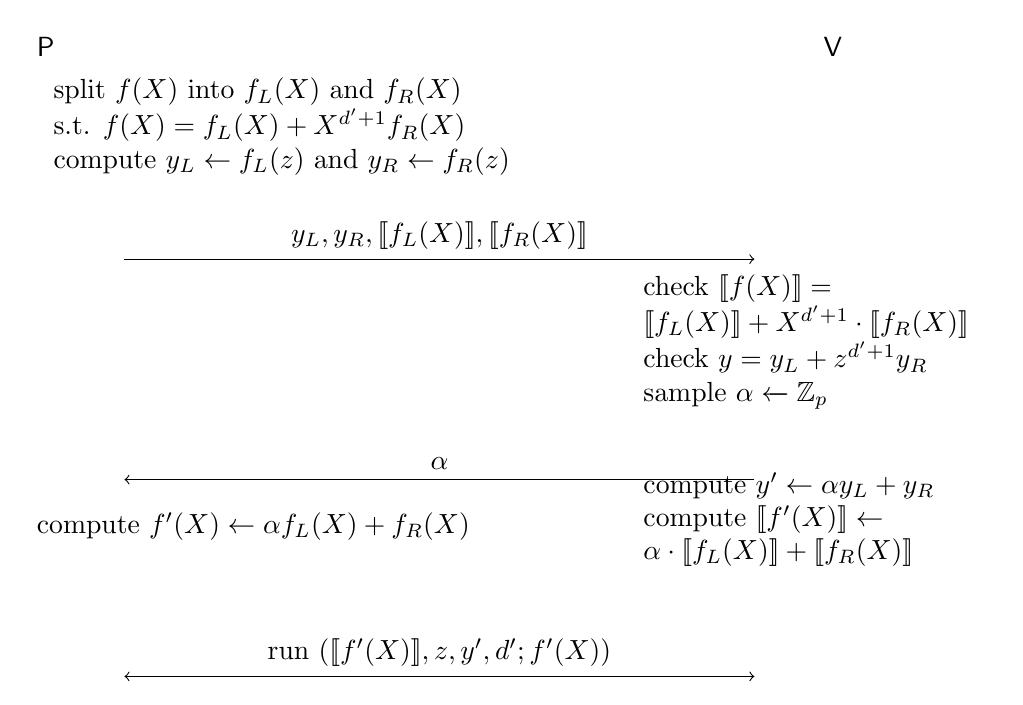
\begin{tikzpicture}
			\node[] (prover) at (-5, 0) {\prover};
			\node[] (verifier) at (5, 0) {\verifier};
			\node[anchor=north west] (prover computes) at (prover.south west) {\begin{tabular}{l}
				split $f(X)$ into $f_L(X)$ and $f_R(X)$ \\
				s.t. $f(X) = f_L(X) + X^{d'+1}f_R(X)$ \\
				compute $y_L \gets f_L(z)$ and $y_R \gets f_R(z)$
			\end{tabular}};
			\draw[->] (-4, -2.7) -- (4, -2.7) node[above, midway] {$y_L, y_R, [\![f_L(X)]\!], [\![f_R(X)]\!]$};
			\node[anchor=north west, xshift=-2.5cm, yshift=-2.5cm] (verifier checks) at (verifier.south west) {\begin{tabular}{l}
			check $[\![f(X)]\!] =$ \\
			 $[\![f_L(X)]\!] + X^{d'+1}\cdot [\![f_R(X)]\!]$ \\
			check $y = y_L + z^{d'+1}y_R$ \\
			sample $\alpha \xleftarrow{\dollar} \mathbb{Z}_p$
			\end{tabular}};
			\draw[->] (4, -5.5) -- (-4, -5.5) node[above, midway] {$\alpha$};
			\node[anchor=north west, yshift=-0.5cm] (verifier updates) at (verifier checks.south west) {\begin{tabular}{l}
				compute $y' \gets \alpha y_L + y_R$ \\
				compute $[\![f'(X)]\!] \gets$ \\
				$\alpha \cdot [\![f_L(X)]\!] + [\![f_R(X)]\!]$
			\end{tabular}};
			\node[anchor=north west, yshift=-4cm] (prover updates) at (prover computes.south west) {compute $f'(X) \gets \alpha f_L(X) + f_R(X)$};
			\draw[<->] (4, -8) -- (-4, -8) node[above, midway] {run $\eval([\![f'(X)]\!], z, y', d'; f'(X))$};
			\end{tikzpicture}
		\end{itemize}
		\end{flushleft}
\end{minipage}
\end{mdframed}
\end{figure}
\end{comment}

\begin{comment}
These operations give rise to the following informal pseudocode description of the \eval protocol.
\begin{mdframed}
Information-theoretic $\eval$ protocol, informal. \\
Common knowledge: $[\![f(X)]\!], y, z, d$ \\
Secret knowledge for \prover: $f(X)$ of degree $d$ \\
Statement: $y = f(z) \bmod p$ and $\deg(f(X)) = d$
	\begin{itemize}[nolistsep]
	    \item \textbf{if} $d > 0$ \textbf{then:}
		\item \pcind[1] \prover splits $f(X)$ into polynomials $f_L(X)$ and $f_R(X)$ of degree $d'=\frac{d+1}{2}-1$ such that $f(X) = f_L(X) + X^{d'+1}f_R(X)$
		\item \pcind[1] \prover sends $[\![f_L(q)]\!]$ and $[\![f_R(q)]\!]$ as well as $y_L \gets f_L(z) \bmod p$ and $y_R \gets f_R(z) \bmod p$ to \verifier
		\item \pcind[1] \verifier checks that $[\![f_L(q)]\!]+q^{d'+1} [\![f_R(q)]\!] = [\![f(q)]\!]$ and $y_L+z^{d'+1} y_R =y$
		\item \pcind[1] \verifier sends a random challenge $\alpha$ from $[-\frac{p-1}{2} ; \frac{p-1}{2}]$ to \prover
		\item \pcind[1] \prover and \verifier recurse on $[\![f'(q)]\!]=\alpha [\![f_L(q)]\!]+[\![f_R(q)]\!]$ for the statement $f'(z) = \alpha y_L + y_R \bmod p$ and $\deg(f'(X)) = d'$
		\item \textbf{if} $d=0$ \textbf{then:}
		\item \pcind[1] $\prover$ sends the constant $f$ to $\verifier$
		\item \pcind[1] $\verifier$ checks that $f$ is a small constant, that $[\![*]\!]$ evaluated in $f$ equals $[\![f]\!]$, and that $y = f \bmod p$
	\end{itemize}
\end{mdframed}
\end{comment}

\subsection{Integer Polynomial Encoding (Ben's version)}
\label{sec:encoding}
We propose using integer commitments in a group of unknown order.as a concrete instantiation of the homomorphic commitment scheme required for the abstract protocol presented in Section~\ref{sec:abstraction}. At the heart of our protocol is thus an encoding of integer polynomials with bounded coefficients as integers, which also has homomorphic properties. 

In order to encode polynomials over an odd prime field $\mathbb{F}_p$, we first lift them to the ring of polynomials over the integers. In the technical overview (Section~\ref{sec:overview}) we noted that a polynomial $f \in \mathbb{F}_p[X]$ can be uniquely encoded as an integer by first mapping $f$ to an integer polynomial $\tilde{f}$ with coefficients in $[0, p)$ and then to the integer $\tilde{f}(q)$ for any $q > p$. 
The coefficients of $f$ can be recovered via the base $q$ decomposition of $\tilde{f}(q)$. 
This encoding is an injective mapping from polynomials in $\FF_p[X]$ of degree at most $d$ to the set $[0, q^d)$. However, this integer encoding is not homomorphic: given $f, g \in \FF_p[X]$ with coefficients greater than $p/2$ the encoding of the polynomial $h \leftarrow f + g \bmod p$, \emph{i.e.} the integer $\tilde{h}(q)$, is distinct from $\tilde{f}(q) + \tilde{g}(q)$. 

In order to make the encodings homomorphic, one approach is to consider any integer $z \in [0, q^{d+1}] $ a valid encoding of $f$ as long as there exists an integer polynomial $f^* \in \ZZ[X]$ with positive coefficients less than $q$ such that $f^*(q) = z$ and $f^* \equiv f \bmod p$. Encodings are no longer unique as there are multiple valid ways to encode the same polynomial in $\ZZ_p[X]$, but encodings are still injective: for any $z$ there is a unique polynomial $f^*$ with positive coefficients less than $q$ such that $f^*(q) = z$ and $f^* \bmod p$ uniquely fixes $f$. 
 Now if the coefficients of $f$ and $g$ are bounded by $q/2$ then $\tilde{f} + \tilde{g} \equiv \tilde{h} \bmod p$, hence $\tilde{h}(q)$ is a valid encoding of $h$. By choosing a sufficiently large $q$ it is possible to perform several levels of homomorphic operations on encodings. 
 
However, this simple change introduces a problem for the protocol in Section~\ref{sec:overview}. The commitments are never checked (i.e. opened) until the bottom level of recursion. Hence, when using integer commitments over this \emph{restricted set of valid} integer encodings, the validity of internal commitments is never verified directly. Moreover, the validity of these internal commitments cannot be infered from the commitment opened at the bottom level of recursion. The integer $f'(q)$ can be written two different ways as $\alpha f_L(q) + f_R(q)$ and $\alpha f_L^*(q) + f_R^*(q)$ for $f^*_L \not \equiv f_L \bmod p$ and $f_R^* \not \equiv f_R \bmod p$ by choosing either $f_L^*$ or $f_R^*$ with negative coefficients. To illustrate this over the degree-0 polynomials at the bottom level, set $\alpha = 1$ and let $f' = 5$, $f_L = 2$, $f_R = 3$, $f_L^* = -1$, and $f^*_R = 6$. At the previous level, the prover could have committed to integer encodings of either the polynomials $3X + 2$ or $6X - 1$. The core issue is that we cannot infer from the fact that $f'(X)$ has \emph{positive} coefficients that the provers commitments $[\![f_L(X)]\!]$ and $[\![f_R(X)]\!]$ were also to integer polynomials with \emph{positive} coefficients. 

Fortunately, from the value of $f'$ we can infer a \emph{probabilistic bound} on the absolute value of the $f_L$ and $f_R$ given that $\alpha \in (-p/2, p/2)$ is sampled randomly \emph{after} the prover has committed to $f_L$ and $f_R$. If $\alpha$ were not chosen randomly by the verifier no bound would apply: knowing $\alpha$, the prover can choose large $f_L$ and $f_R$ such that $\alpha f_L + f_R$ is small. The probabilistic bound is reasoned as follows: if $f'_0 \leftarrow \alpha_0 f_L + f_R$ and $f'_1 \leftarrow \alpha_1 f_L + f_R$ such that $max(|f'_0|, |f'_1|) < q / (2p)$ for some distinct $\alpha_0 \neq \alpha_1$, then $|f_L| \geq |f'_1 - f'_0| \leq q / p$ and $|f_R| \leq |\alpha_0 f'_1 - \alpha_1 f'_0| \leq q/2$. If no such pair exists, \emph{i.e.} the bound only holds for a unique $\alpha$, then there is a negligibly small probability $1/p$ that $f'$ would have passed the bound check. 
More generally, a bound on $||f'(X)||_\infty$ in some level of the recursion implies a probabilistic bound on $||f_L(X)||_\infty$ and $||f_R(X)||_\infty$ at the previous level. (For a polynomial $g \in \ZZ[X]$ the norm $||g||_\infty$ is the maximum over the absolute values of all individual coefficients of $g$).

This leads us to the following encoding scheme. We restrict the set of \emph{valid} encodings to be integers in the range $B = (-\frac{q^{d+1}}{2}, \frac{q^{d+1}}{2})$. An integer $z \in B$ is a valid encoding of $f \in \ZZ_p[X]$ if and only if there exists $\tilde{f} \equiv f \bmod p$ such that $||\tilde{f}||_\infty < q/2$ and $\tilde{f}(q) = z$. Every $z \in B$ encodes a unique $f \in \FF_p[X]$ of degree at most $d$. (We prove this fact below). 

\paragraph{Encoding scheme} Let $\ZZ(b):=\{x \in \ZZ: \vert x \vert  \leq b\}$ denote the set of integers with absolute value less than or equal to $b$. Define $\ZZ(b)[X] := \{f \in \ZZ[X]: ||f||_\infty \leq b\}$, the set of integer polynomials with coefficients from $\ZZ(b)$. 

\begin{itemize} 

\item \textbf{Encoding.}
For any integer $q$, the function $\mathsf{Enc} : \mathbb{Z}(b)[X] \rightarrow \mathbb{Z}$ maps $h(X) \mapsto h(q)$. A polynomial $f(X) \in \ZZ_p[X]$ is first mapped to $\ZZ(p/2)[X]$ by replacing each coefficient of $f$ with its unique integer representative from $(-p/2,p/2)$ of the same equivalence class modulo $p$.  %This means the map can be used as encoding of polynomials in the domain $\ZZ(b)[X]$ with $b<q/2$.

\item \textbf{Decoding.}
Decoding works as follows. Define the partial sum $S_k := \sum_{i=0}^k f_i q^i$ with $S_{-1} := 0$. Assuming $|f_i| < q/2$ for all $i$, observe that for any partial sum $S_k$ we have $|S_k|<\frac{q^{k+1}}{2}$. Therefore, when $S_k < 0$ then $S_k \bmod q^{k+1} > q^{k+1}/2$ and when $S_k \geq 0$ then $S_k \bmod q^{k+1} < q^{k+1}/2$. 
This leads to a decoding strategy for recovering $S_k$ from $y \in \mathbb{Z}$. The decode algorithm sets $S_k$ to $y \bmod q^{k+1}$ if this value is less than $q^{k+1}/2$ and to $q^{k+1}- (y \bmod q^{k+1})$ otherwise.
Two consecutive partial sums yield a coefficient of $f(X)$: $f_k = \frac{S_{k} - S_{k-1}}{q^{k}} \in \ZZ(b)$. These operations give rise to the following algorithm.\\
\end{itemize}

 \begin{minipage}{\textwidth}
\begin{mdframed}
\begin{flushleft}
	$\pro{Dec}(y \in \mathbb{Z}):$
	\begin{enumerate}[nolistsep]
	    \item \textbf{for each} $k$ \textbf{in} $[0, \, \lfloor \log_q(|y|)\rfloor]$ \textbf{do:}\\
		\item \pcind[1] $S_{k-1} \gets (y \bmod q^{k})$
		\item \pcind[1] \pcif{$S_{k-1} > q^{k}/2$} \textbf{then} $S_{k-1} \gets q^{k}-S_{k-1}$ \textbf{end if}
		\item \pcind[1] $S_k \gets (y \bmod q^{k+1})$
		\item \pcind[1] \pcif{$S_{k} > q^{k+1}/2$} \textbf{then} $S_{k} \gets q^{k+1}-S_{k}$ \textbf{end if}
		\item \pcind[1] $f_k \gets (S_{k} - S_{k-1}) / q^k$
		\item \pcreturn $f(X) = \sum_{k=0}^{\lfloor \log_q(|y|)\rfloor} f_k X^k$
	\end{enumerate} 
\end{flushleft}
\end{mdframed}
\end{minipage} \\ 


\subsection{Encoding Polynomials as Integers (Alan's version)}
\label{sec:encoding}

Instantiating the commitment function $[\![*]\!]$ presents two difficulties. First, in terms of size the commitment must be relatively or completely independent of the polynomial it is committing to. Second, despite its compressing nature, the commitment must enable the linear and monomial homomorphisms. Exponentiation in groups of unknown order comes close to solving these issues. A commitment can be a single finite group element, and the message represented thereby cannot be compressed by a malicious adversary because any such compression would rely on knowledge of the group order. Furthermore, the group operation along with re-exponentiation provides useful homomorphisms. Unfortunately, however, the exponentiation map $\mathbb{G} \times \mathbb{Z} \rightarrow \mathbb{G}$ operates on \emph{integers} and not on polynomials over a finite field. Therefore, in order to use this map, we must first find an integer representation of the polynomials we deal with that enables the required homomorphisms.

We consider only polynomials defined over an odd prime field $\mathbb{F}_p$, along with a public parameter $q \gg p$, which is a ``large enough'' integer --- we will determine precisely what ``large enough'' means later on. To represent a polynomial $f(X)$ as an integer, first lift it to the ring of polynomials with integer coefficients by selecting representatives from $\{-\frac{p-1}{2}, \ldots, \frac{p-1}{2}\}$ for each coefficient. Then evaluate the lifted polynomial $\hat{f}(X)$ in $q$.

\paragraph{Negative coefficients.}
Why do we choose representatives from $\{-\frac{p-1}{2}, \ldots, \frac{p-1}{2}\}$, rather than the much more intuitive and accessible choice $\{0, \ldots, p-1\}$? The reason for this alternative choice has to do with a prover's capacity to commit to polynomials with negative coefficients in addition to positive ones.\footnote{Even in a group with infeasible inversion, the computation of an inverse is not needed to commit to $f(X) \in \mathbb{Z}[X]$ with negative coefficients as long as $f(q)$ is positive.}

The commitments are never checked until the last recursion step, where only one commitment is opened. The validity of prior commitments is therefore never verified directly. Moreover, the validity of these earlier commitments cannot be inferred from the commitment opened in the last step. As a result, it is possible for negative coefficients to disappear in the course of the protocol, for instance if they are added to positive coefficients that are larger in absolute value. Likewise, it is possible for large coefficients to shrink in the course of the protocol.

To complicate matters further, it is possible that for some polynomial $f^*(X)$ with negative coefficients, $f^*(q) = f(q)$ but $f^*(X) \not \equiv f(X) \bmod p$, for instance if $f^*(X) - f(X)$ is a polynomial-multiple of $X-q$. The combined effect is that \emph{a malicious prover can continue with a different polynomial modulo $p$, and bank on the rather likely event that the negative coefficients will disappear in the course of the protocol.}

The solution to this problem is for the verifier to check that the opening of the last commitment belongs to a \emph{bounded interval} whose cardinality is much smaller than $q$. While it is possible for small coefficients to disappear, and for large ones to shrink, the point is that such events are difficult to anticipate for a prover who does not know $\alpha$ ahead of time. Moreover, a malicious prover looking to exploit the single commitment to two polynomials $f^*(X)$ and $f(X)$ with $f^*(X) \not \equiv f(X) \bmod p$ but $f^*(q) = f(q)$ must use polynomials that have coefficients on the order of magnitude of $q$ somewhere. With overwhelming probability, these large coefficients will percolate to the final step of the protocol where they fail the bound test, thereby exposing the fraud.

%The choice to select representatives for $\mathbb{Z}_p$ from $\{-\frac{p-1}{2}, \ldots, \frac{p-1}{2}\}$ anticipates a two-fold solution to address this problem. First, in a balanced $q$-ary expansion of some large integer, a coefficient $-a$ (for small $a \in \mathbb{N}$) is identifiable with $p-a \bmod p$ rather than $q-a \bmod p$. As a result, the malicious prover who wants to simultaneously commit to polynomials $f(X)$ and $f^*(X)$ where $f(q) = f^*(q)$ but $f(X) \not \equiv f^*(X) \bmod p$, cannot use small negative coefficients alone and must additionally use coefficients on the order of magnitude of $q$ in absolute value. Second, in the last step of the protocol when the last commitment is opened, the verifier will check if the transmitted integer belongs to a \emph{bounded interval}. If at any point the prover was using two polynomials $f(X)$ and $f^*(X)$ such that $f(q) = f^*(q)$ but $f(X) \not \equiv f^*(X) \bmod p$, then some coefficients had to be large in absolute value, and with overwhelming probability those large coefficients percolate to the final step where they fail the bound test. 

While it is possible to adapt the bound test for strictly positive integers --- matching a standard, non-balanced set of representatives --- the point is that this bound works by checking the integer's magnitude. From this perspective, a balanced set of representatives for the coefficients of $f(X)$ and for $\alpha$ is the more natural choice and conveniently simplifies the security proof in several locations. This choice matches with the intuition that a small negative coefficient is more likely to disappear than a large one, positive or negative.

\paragraph{Encoding Scheme}

We write $\ZZ(b):=\{x \in \ZZ \, | \, \vert x \vert  \leq b\}$ as the set of integers with absolute value less than or equal to $b$. In a slight abuse of notation we write $\ZZ(b)[X]\subset \mathbb{Z}[X]$ as the set of integer polynomials with bounded coefficients. Additionally, we will identify $\mathbb{Z}_p[X]$ with $\mathbb{Z}(p)[X]$ and use the hat-notation $\hat{f}(X)$ only when it is necessary to make the type distinction explicit.

\begin{itemize}
    \item \textbf{Encoding}
For a ``large'' integer $q$, the map $\mathsf{Enc} : \mathbb{Z}((q-1)/2)[X] \rightarrow \mathbb{Z}, \, f(X) \mapsto f(q)$ is an injective map from polynomials with bounded coefficients to the integers. This means the map can be used as encoding of polynomials in the domain $\ZZ(b)[X]$ with $b<q/2$.
    \item \textbf{Decoding}
Decoding works as follows. Define the partial sum $S_k := \sum_{i=0}^k f_i q^i$ with $S_{-1} := 0$ and observe that when $(S_k \bmod q^{k+1}) > q^{k+1}/2$ then $S_k < 0$ whereas when $(S_k \bmod q^{k+1}) < q^{k+1}/2$ then $S_k \geq 0$. 
So when decoding $y \in \mathbb{Z}$, we can get $S_k$ for any $k$ by setting $S_k$ to $y \bmod q^{k+1}$ if $y \bmod q^{k+1}$ is less than $\frac{q^{k+1}}{2}$ or to $q^{k+1}- (y \bmod q^{k+1})$ otherwise.
Two consecutive partial sums yield a coefficient of $f(X)$: $f_k = \frac{S_{k} - S_{k-1}}{q^{k}} \in \ZZ(b)$. These operations give rise to the following algorithm.\\
\begin{minipage}{0.9\textwidth}
\begin{mdframed}
\begin{flushleft}
	$\pro{Dec}(y \in \mathbb{Z}):$
	\begin{enumerate}[nolistsep]
	    \item \textbf{for each} $k$ \textbf{in} $[0, \, \lfloor \log_q(|y|)\rfloor]$ \textbf{do:}\\
		\item \pcind[1] $S_{k-1} \gets (y \bmod q^{k})$
		\item \pcind[1] \pcif{$S_{k-1} > q^{k}/2$} \textbf{then} $S_{k-1} \gets q^{k}-S_{k-1}$ \textbf{end if}
		\item \pcind[1] $S_k \gets (y \bmod q^{k+1})$
		\item \pcind[1] \pcif{$S_{k} > q^{k+1}/2$} \textbf{then} $S_{k} \gets q^{k+1}-S_{k}$ \textbf{end if}
		\item \pcind[1] $f_k \gets (S_{k} - S_{k-1}) / q^k$
		\item \pcreturn $f(X) = \sum_{k=0}^{\lfloor \log_q(|y|)\rfloor} f_k X^k$
	\end{enumerate} 
\end{flushleft}
\end{mdframed}
\end{minipage}
\end{itemize}
	
\begin{lemma}
If $b < \frac{q}{2}$, then for all polynomials $f(X) \in \mathbb{Z}(b)[X]$, $\mathsf{Dec}(\mathsf{Enc}(f(X))) = f(X)$.
\end{lemma}

\begin{proof}
The encoding $\mathsf{Enc}$ is injective for $\mathbb{Z}(b)$ because any colliding pair of polynomials $f(X)$, $g(X)$ such that $\mathsf{Enc}(f(X)) = \mathsf{Enc}(g(X))$ differ by a multiple of $X-q$. This implies that either $f(X)$ or $g(X)$ must have a coefficient larger than or equal to $\frac{q}{2} > b$ in absolute value. What remains to be shown is the correctness of decoding, and this follows from the observation that re-encoding the decoded polynomial $\bar{f}(X) = \mathsf{Dec}(\mathsf{Enc}(f(X))$ gives $\mathsf{Enc}(f(X))$. By construction: $\mathsf{Enc}(\bar{f}(X)) = \sum_{k=0}^{\lfloor \log_q(|y|) \rfloor} f_k q^k = S_{\lfloor \log_q (|y|) \rfloor} = y = f(q) = \mathsf{Enc}(f(X))$.
\end{proof}

Note that the encoding has limited homomorphic properties: $\enc(g(X))+\enc(h(X))=\enc(g(X)+h(X))$ if $g(X)+h(X)\in \ZZ(b)$. This constraint is satisfied, for example, if all coefficients are less than $b/2$ in magnitude and $b < q/2$. Additionally, $\enc(g(X))\cdot \enc(h(X))=\enc(g(X)\cdot h(X))$ if $g(X)\cdot h(X)\in \ZZ(b)$.

\paragraph{Encoding of dyadic rational polynomials.}
There exists an algorithm to compute square roots of any element of a class group of an imaginary quadratic order, originally described by Gauß (see Bosma and Stevenhagen for a modern description~\cite{jtn/BosSte96}). As a result, in such class groups an adversary can also commit to \defn{dyadic rationals} $\mathbb{D}:=\{\frac{x}{2^k} : \ x \in \ZZ \wedge k \in \NN\}\subset \QQ$, in addition to integers. When using class groups we therefore need to modify the encoding scheme . 

The encoding map is identical, except lifted to the dyadic rationals: $\mathsf{Enc} : \mathbb{D}[X] \rightarrow \mathbb{D}, \, g(X) \mapsto g(q)$. The main difference with respect to the integer encoding scheme will be that decoding works for dyadic rationals where \emph{both the numerator and the denominator are bounded}. Let $N \in \NN$ be a bound on the absolute value of the numerator and $2^D\in \NN$ be a bound on the value of the denominator, and let $\mathbb{D}(N, D) :=\{\frac{x}{2^a} \in \mathbb{D} : \ |x|\leq N \wedge 2^a \leq D\}$ denote the set of such bounded dyadic rationals. The encoding scheme is uniquely decodable if $N \cdot 2^a < q/2$.
 
Note that denominator of $g(q)$ is bounded by $2^{\lfloor\log_2(D)\rfloor}$, $D$ rounded down to the next power of $2$. To decode such a dyadic rational, compute the integer $y \gets g(q) \cdot 2^{\lfloor\log_2(D)\rfloor}\in \ZZ$  and use the decoding algorithm described above to decode a polynomial $f(X)$ in $\ZZ(q/2)[X]$. From $f(X)$ one derives the polynomial  $g(X) \gets \frac{f(X)}{2^{\lfloor\log_2(D)\rfloor}} \in \mathbb{D}(\lceil q/(2D)\rceil, 2^{\lfloor\log_2(D)\rfloor})[X]$ through division. If the integer polynomial encoding is uniquely decodable, then so is the scheme for dyadic rational polynomials. If $q$ is a power of $2$, then an adversary can encode Laurent polynomials, \emph{i.e.}, polynomials where some terms have negative powers. In order to disallow negative powers, $q$ must be odd.

\subsection{Concrete Polynomial Commitment Scheme}

We now instantiate the abstract homomorphic commitment function $[\![ * ]\!]$. To this end we sample a group of unknown order $\mathbb{G}$, and sample a random element $\gr{g}$ from this group. 
Lift the field polynomial $f(X)\in \ZZ_p[X]$ to an integer polynomial with bounded coefficients, \emph{i.e.}, $\hat{f}(X)\in \ZZ(\frac{p-1}{2})[X]$ such that $\hat{f}(X)\bmod p=f(x)$.
We encode $\hat{f}(X)$ as an integer by evaluating it at a ``large enough'' integer $q$. Finally we use exponentiation in $\GG$ to commit to the integer. $[\![f(X)]\!]$, therefore, corresponds to $\gr{g}^{\hat{f}(q)}$. This commitment function inherits the homomorphic properties of the integer encoding for a limited number of additions and multiplications-by-constant. The monomial homomorphism for $X^d$ is achieved by raising the group element to the power $q^{d}$. To maintain consistency between the prover's witness polynomials and the verifier's commitments, the prover operates on polynomials with integer coefficients  $\hat{f}(X), \hat{g}(X)$, \emph{etc.}, without ever reducing them modulo $p$.

The $\setup, \pro{Commit}$ and $\open$ functionalities are presented formally below. Note that the scheme is parameterized by $p$ and $q$.
%; these values are determined by the context and independently of $\setup$.

%We now present our main technical contribution: a polynomial commitment scheme with an efficient evaluation protocol based on a group of unknown order $\GG$. For polynomials of degree $d=\poly$ the evaluation protocol uses $1+\lceil\log_2(d+1)\rceil$ rounds and $O(\log(d))$ communication and verifier work.

%Exponentiation in groups of unknown order is a succinct and homomorphic cryptographic commitments to an integer.
%Using the integer encoding of polynomials, or their encoding as dyadic rationals, above we can simply commit to a polynomial $f(X)$ with bounded coefficients by computing $\gr{g}^{f(q)} \in \GG$. Every polynomial in $\ZZ_p[X]$ naturally maps to an integer polynomial with coefficients in $B_{\frac{p-1}{2}}$. The commitment scheme, therefore, supports committing to polynomials in $\ZZ_p[X]$ for $p \leq q$. Interestingly, neither $p$ nor the degree $d$ need to be specified in the setup. 

%As long as $q$ and ``big enough'' they can be freely chosen.\alan{Todo: make this observation elsewhere.} %In class groups there is an efficient algorithm to compute square roots, and as a result, a prover can also commit to dyadic rationals. Since every dyadic rational corresponds to a unique element in $\ZZ_p$ we can simply extend the encoding to work for polynomials with bounded dyadic rational coefficients. The only difference is that we require $q$ to be odd such that the prover cannot commit to polynomials with negative powers. We will discuss the relationship between $p$, $d$ and $q$ in more detail later but first we describe the setup, commitment and opening algorithms:

\begin{itemize}
\item $\pro{Setup}(1^\secpar):$ Sample $ \GG \sample \ggen(\secpar)$
			and $ \gr{g} \sample \GG$. Return $\params = (\secpar,\GG,\gr{g}, q)$.
\item $\pro{Commit}(\params;f(X) \in \ZZ_p[X]):$ Compute $\gr{C} \gets \gr{g}^{\hat{f}(q)}$ and return $(\gr{C};\hat{f}(X))$.
\item $\pro{Open}(\params,\gr{C}, f(X), \hat{f}(X)):$ Check that $\hat{f}(X)\in \ZZ(q/2)[X]$ and $\gr{g}^{\hat{f}(q)} = \gr{C}$ and $f(X) = \hat{f}(X) \bmod p$. 
\end{itemize}

\begin{comment}
\begin{small}
\begin{mdframed}[userdefinedwidth=\textwidth]
\begin{minipage}{\textwidth}
	\begin{flushleft}
	$\pro{Setup}(1^\secpar):$
		\begin{enumerate}[nolistsep]
			\item $ \GG \sample \ggen(\secpar)$
			\item $ \gr{g} \sample \GG$
			%\item $q \gets 2^k$ such that $q > (d+1) \cdot 2\cdot p^{\log_2(d+1)+1} $
			%\item Pick a prime $p\in \NN$ such that $\lceil\log_2(p)\rceil=\lambda$.
			%\item Pick a sufficiently large and odd $q\in \NN$ (See discussion above)
			%\item $\pcreturn \params = (\secpar,\GG,\gr{g},p,q)$
			\item $\pcreturn \params = (\secpar,\GG,\gr{g})$
		\end{enumerate}
	$\pro{Commit}(\params;f(X) \in \ZZ(p)[X]):$ \pccomment{$f(X)\equiv \bar{f}(X) \mod p$ for  $\bar{f}(X)\in \ZZ_p[X]$}
		\begin{enumerate}[nolistsep]
			\item $\gr{C} \gets \gr{g}^{f(q)}$
			\item $\pcreturn (\gr{C};f(X))$
		\end{enumerate}
	$\pro{Open}(\params,\gr{C}, f(X)):$ \pccomment{$f(X) \in \ZZ(b)[X]\subset\mathbb{Z}[X]$ for $b<q/2$}
		\begin{enumerate}[nolistsep]
		    \item \prover sends $f(X)$ to \verifier.
		   % 				\item \verifier checks that $\bar{f}(X) = f(X) \mod p$
		    \item \verifier checks that $f(X)\in \ZZ(b)[X]$ and $b<q/2$
			\item \verifier checks that $\gr{g}^{f(q)} = \gr{C}$ \pccomment{Can be outsourced using $\textsf{PoE}(\gr{g},\gr{C},f(q))$}
			\item \pcif all checks pass \textbf{then} \pcreturn $1$ \textbf{else} \pcreturn $0$
		\end{enumerate}
		\end{flushleft}
\end{minipage}
\end{mdframed}
\end{small}
\end{comment}
%Opening the commitment can be simply done by rerunning the commitment algorithm. Additionally a proof of exponentiation (PoE) can be used to increase verifier efficiency.
%The commitment inherits the homomorphic properties of the integer encoding. Assume that we are committing to representations of polynomials in $\ZZ_p[X]$, \emph{i.e.}, polynomials with coefficients bounded by $p$. Then the commitment scheme supports up to $\frac{q}{p}$ homomorphic additions. Equivalently, when raising a commitment to a weight $\alpha$, the size of the coefficients grows by at most a factor of $|\alpha|$. We use this property to build an efficient $\eval$ protocol. 

%The core idea of the $\eval$ protocol is to reduce the statement from one about a polynomial $f(X)$ of degree $d$ to one about a polynomial of degree $d'=\frac{d+1}{2}-1$. For simplicity assume that $d+1$ is a power of $2$.
%The prover splits $f(X)$ into $f_L(X)$ and $f_R(X)$ such that $f(X) = f_L(X)+X^{d'+1} f_R(X)$ and such that both polynomials have degree at most $d'$. Then he proves that $f'(X)=\alpha \cdot f_L(X) + f_R(X)$ has degree $d'$ for a random challenge $\alpha\in [-\frac{p-1}{2},\frac{p-1}{2}]$. 

%If the prover wants to show, in addition to the previous, that $f(z)=y\bmod p$, then he can simply provide $y_L=f_L(z)\bmod p$ and $y_R=f_R(z)\bmod p$ and show that $y_L + z^{d'+1} \cdot y_R \bmod p=y$. Note that the verifier can compute $y' = f'(z) = \alpha \cdot y_L + y_R \bmod p$ from $y_L$ and $y_R$.

%The proof recursively repeats this reduction by using $f'(X),z,y'$ and $d'$ as the input. In the final step, the prover simply sends the constant polynomial $f$ and the verifier can check that $f \equiv y \bmod p$. Note that $|f|< (\frac{p}{2})^{\log_2(d+1)+1}$ so an integer encoding of $f_0$ requires at most $\lceil \log_2(d+1) \cdot \log_2(p)\rceil$ bits. 
\paragraph{Evaluation protocol}
Using the cryptographic compilation of the information theoretic protocol we get an $\eval$ protocol with logarithmic communication. In every round, however, the verifier needs to check consistency between $[\![f_L(X)]\!],[\![f_R(X)]\!]$ and $[\![f(X)]\!]$. This is done by checking that $\gr{C}_L \cdot \gr{C}_R^{q^{d'+1}}=\gr{C}$. This naive check is highly inefficient as the exponent $q^{d'+1}$ has $O(d)$ bits.
%For the concrete evaluation protocol, one starts with the situation in which the verifier possesses a commitment to $f(X)$ in the form of $\gr{C} = \gr{g}^{f(q)}$. The prover commits to $f_L(X)$ and $f_R(X)$ by sending $\gr{C}_L$ and $\gr{C}_R$. The verifier checks that $\gr{C} = \gr{C}_L \cdot \gr{C}_R^{q^{d'+1}}$ and proceeds in the next step with the commitment $\gr{C}' = \gr{C}_L^\alpha \cdot \gr{C}_R$ to $f'(X)$. This instantiation produces an $\eval$ protocol with logarithmic communication. However, naïvely checking that $f(X) = f_L(X) + X^{d'+1} f_R(X)$ based on the commitments $\gr{C}, \gr{C}_L$ and $\gr{C}_R$ is inefficient because the bit-size of the exponent $q^{d'+1}$ is huge.
To resolve this inefficiency, we utilize a proof of exponentiation (\textsf{PoE})~\cite{ITCS:Pietrzak18,EC:Wesolowski19} to outsource the computation to the prover.
The \textsf{PoE} protocol is an argument that a large exponentiation in a group of unknown order was performed correctly. Wesolowski's \textsf{PoE}~\cite{EC:Wesolowski19} is public coin, has constant communication and verification time, and is thus particularly well-suited here.

We now specify subtleties that were previously glossed over. 
First, we handle the case where $d+1$ is not a power of 2.  Whenever $d+1$ is odd in the recursion, the polynomial is shifted by one degree --- specifically, $f'(X) = X f(X)$ and the protocol proceeds to prove that $f'(X)$ has degree bounded by $d' = d+1$ and evaluates to $y' = zy$ at $z$. The verifier obtains the matching commitment $\gr{C}'\gets\gr{C}^q$.

Second, the coefficients of $f(X)$ grow by a factor of $\frac{p+1}{2}$ in every recursion step, but eventually the transmitted constant $f$ has to be tested against some bound because if it is \emph{too large} it should be rejected. However, the function interface provides no option to specify the allowable size of coefficients. We therefore define and use a subroutine $\pro{EvalBounded}$, which takes an additional argument $b$ and which proves, in addition to what $\pro{Eval}$ proves, that all coefficients $f_i$ of $f(X)$ satisfy $|f_i| \leq b$. Importantly, $b$ grows by a factor for $\frac{p+1}{2}$ in every recursion step. This subroutine is also useful if commitments were homomorphically combined prior to the execution of $\pro{EvalBounded}$. The growth of these coefficients determines a lower bound on $q$: $q$ should be \emph{significantly} larger than $b$. Exactly which factor constitutes ``significantly'' is determined by the knowledge-soundness proof.

In the final round we check that the constant $f$ satisfies $|f|\leq b$ and the protocol's correctness is guaranteed if $b = \frac{p-1}{2}(\frac{p+1}{2})^{\lceil\log_2(d+1)\rceil}$. However, $q$ needs to be even larger than this value in order for extraction to work (and hence, for the proof of witness-extended emulation to go through). In RSA groups, where computing square roots is hard, we need $q>p^{2\log(d)}$; whereas in class groups where computing square roots is easy, we need $p^{3\log(d)}$. When this condition is satisfied, we can prove that the original committed polynomial has coefficients smaller than $\frac{q}{2}$. To avoid presenting two algorithms whose only difference is the one constant, we capture this constant explicitly in the variable $\boldsymbol{\varsigma}_{p,d}$ and set its value depending on the context:
\[
    \boldsymbol{\varsigma}_{p, d} = \left\{
        \begin{array}{ll}
            p^{\,2\log_2(d+1)} & \quad \textnormal{(in RSA groups)} \\
            p^{\,3\log_2(d+1)} & \quad \textnormal{(in class groups)}
        \end{array}
    \right. \enspace .
\]

 We now present the full, formal $\eval$ protocol below.
\begin{small}
\begin{mdframed}
\begin{minipage}{\textwidth}
			$\pro{Eval}(\crs, \gr{C}\in \GG, z\in \ZZ_p, y\in \ZZ_p, d \in \NN; \bar{f}(X)\in \ZZ_p[X]) :$ \pccomment{$\bar{f}(X) = \sum_{i=0}^d \bar{f}_i X^i$}
			\begin{enumerate}[nolistsep]
			\item \prover computes $f_i \in [-\frac{p-1}{2},\frac{p-1}{2}]$ such that $f_i\equiv \bar{f}_i\bmod p$ for all $i\in[0,d]$.
			\item \prover computes $f(X)\gets \sum_{i=0}^d f_i \cdot X^{i}\in \ZZ(p)[X]\subset \ZZ[X]$
			\item \prover and \verifier run $\pro{EvalBounded}(\params,\gr{C},z,y,d,\frac{p-1}{2};f(X))$
		    \end{enumerate}
		    		\vspace{1em}
		$\pro{EvalBounded}(\crs,\gr{C}\in \GG,z\in \ZZ_p,y\in \ZZ_p,d\in \NN,b\in \ZZ;f(X)\in \ZZ(b)[X])$		
	    \begin{enumerate}[nolistsep]
        \item \pcif $d=0$:
        \item \label{line:basestart}\pcind[1] \prover sends $f(X)\in \ZZ$ to the verifier. \pccomment{$f=f(X)$ is a constant}
        \item \pcind[1] \verifier checks that $b\cdot \boldsymbol{\varsigma}_{p,d} < q$\pccomment{$\boldsymbol{\varsigma}_{p,d}$ is $p^{2\log_2(d+1)}$ or $p^{3\log_2(d+1)}$ depending on context.}
        %q/(2^{\lceil \log_2(d+1) \rceil+1} p^{2 \lceil \log_2(d+1) \rceil+1})$
        \item \pcind[1] \verifier checks that $|f|\leq b$
          \item \pcind[1] \verifier checks that $f\equiv y \bmod p$
                \item \label{line:baseend}\pcind[1] \verifier checks that $\gr{g}^{f}=\gr{C}$
\item \pcind[1] \verifier outputs $1$ \pcif all checks pass, $0$ otherwise.
          \item \pcif{$d+1$ is odd}
         \item \pcind[1]  $d'\gets d+1, \gr{C}'\gets \gr{C}^q$, $y'\gets y\cdot z \bmod p$ and $f'(X)\gets X \cdot f(X)$.
         \item \pcind[1] \prover and \verifier run $\pro{EvalBounded}(\crs,\gr{C}',z,y',d',bd;f'(X))$

        \item \pcelse: \pccomment{$d \geq 1$ and $d+1$ is even}
       
        \item \pcind[1] \prover and \verifier compute $d' \gets \frac{d+1}{2} - 1$
        \item \pcind[1] \prover computes $f_L(X) \gets \sum\limits_{i=0}^{d'} f_i \cdot X^i$ and $f_R(X)\gets\sum\limits_{i=0}^{d'} f_{d'+1+i}\cdot X^{i}$
        \item \pcind[1] \prover computes $y_L\gets f_L(z) \bmod p$ and $y_R\gets f_R(z)\bmod p$
        \item \pcind[1] \prover computes $\gr{C}_L \gets \gr{g}^{f_L(q)}$ and $\gr{C}_R \gets \gr{g}^{f_R(q)}$
        \item \pcind[1] \prover sends $y_L,y_R, \gr{C}_L, \gr{C}_R$ to \verifier. \pccomment{See Section \ref{subsec:optimization} for an optimization}
        \item \pcind[1] \verifier checks that $y=y_L+z^{d'+1}\cdot y_R \bmod p$, outputs $0$ if check fails.
        \item \pcind[1] \label{line:PoE} \prover and \verifier run $\pro{PoE}(\gr{C}_R, \gr{C}/\gr{C}_L, q^{d'+1})$\pccomment{Showing that $\gr{C}_L\gr{C}_R^{(q^{d'+1})}=\gr{C}$}
        \item \pcind[1] \verifier samples $\alpha \sample [-\frac{p-1}{2},\frac{p-1}{2}]$ and sends it to \prover
        \item \pcind[1] \prover and \verifier compute $y'\gets\alpha  y_L +y_R \bmod p$, $\gr{C}' \gets \gr{C}_L^\alpha  \gr{C}_R$, $b'\gets b \frac{p+1}{2}$. 
        \item \pcind[1] \prover computes $f'(X) \gets \alpha \cdot f_L(X) + f_R(X) \in \ZZ[X]$ \pccomment{$\deg(f'(X))=d'$}
        \item \pcind[1] \prover and \verifier run $\pro{EvalBounded}(\params, \gr{C}', z, y', d',b' ; f'(X))$
               \end{enumerate}
      \end{minipage}
\end{mdframed}
\end{small}


\begin{comment}
\end{comment}

\subsection{Security Analysis} 
 \newcommand{\bindinglemma}{
 The polynomial commitment scheme is binding for polynomials in $\ZZ(b)[X]$ for $b<q/2$ if either the Order Assumption or the Strong RSA Assumption hold.
	}
\begin{lemma}
\label{lem:binding}
	\bindinglemma
	\end{lemma}

\newcommand{\correctnesslemma}{
The polynomial commitment scheme is correct for polynomials in $\ZZ_p[X]$ of degree at most $d$ if $q> (p-1) (\frac{p+1}{2})^{\lceil \log_2(d+1)\rceil}$.
}
 
 \begin{lemma}
 	\label{lem:correctness}
\correctnesslemma
 \end{lemma}


The proofs of the previous lemmas are in Appendix~\ref{appendix:binding} and \ref{appendix:correctness}.
Next is the main security theorem, which states that the evaluation protocol has witness-extended emulation. We start with a high-level intuitive overview where we also identify potential obstacles.

\paragraph{Proof idea.} %Consider the information theoretic version of the $\eval$ protocol, where the prover sends the integer polynomials $f_L(X)$ and $f_R(X)$ in each round but the verifier does not read them.
The goal is to construct an extractor by recursively computing $f(X)$ from $f'(X)$. In the final round the verifier receives $f$ such that $|f| \leq b$, and therefore the extractor possesses this constant polynomial as well. Working backwards from here, the extractor uses rewinding in every step to find $f_L(X)$ and $f_R(X)$ and thereby finds $f(X) = f_L(X) + X^{d'+1}f_R(X)$.
Specifically, in each round the extractor has $f'(X)=\alpha f_L(X)+ f_R(X)$. Suppose the extractor also possesses $f''(X)=\alpha' f_L(X)+ f_R(X)$. From $f'(X)$, $f''(X)$, $\alpha$ and $\alpha'$ it is easy to compute $f_L(X)$ and $f_R(X)$. The extractor then computes $f(X)=f_L(X)+X^{d'+1} f_R(X)$.
A careful analysis shows that if the coefficients of $f'(X)$ are bounded by $b$ then $f_L(X)$ and $f_R(X)$ must have coefficients bounded by $b \cdot p$ in absolute value. Using a similar analysis we can show that $f(z)\bmod p=y$ for the extracted polynomial $f(X)$.

This argument shows that there is an extractor algorithm $\mathcal{X}$ capable of extracting the witness $f(X)$ from a binary tree of accepting transcripts. Moreover, a tree-finding algorithm $\mathcal{T}$ can output such a tree by repeatedly rewinding the prover, running it with fresh verifier randomness each time, and recording the resulting transcripts. As a result, the Generalized Forking Lemma (Lemma~\ref{lemma:GFL}) applies and establishes that the protocol has witness-extended emulation.

The full proof takes into account the cryptographic compilation of the protocol using the integer encoding and the commitment scheme based on groups of unknown order. Additionally the full proof will need to support dyadic rationals because taking square roots is easy in class groups.





%We are now in a position to prove the main security statement.

%%%OLD THEOREM
\newcommand{\maintheorem}{
The polynomial commitment scheme for polynomials in $\ZZ_p[X]$ of degree at most $d=\poly$, instantiated using $q>(p-1)(\frac{p^2-1}{2})^{\lceil \log_2(d+1)\rceil}=O(p^{2\log(d)})$ and $\ggen$, has witness extended emulation (Definition \ref{def:wee}) if the Adaptive Root Assumption and the Strong RSA Assumption hold for $\ggen$.
}
\begin{theorem}~\label{thm:polycommitsecurity} 
	\maintheorem
\end{theorem}

%\textit{Remark:}
%The bound on $q$ for correctness (Lemma \ref{lem:correctness}) is $O((\frac{p}{2})^{\log(d)})$ while the bound for soundness is $O((\frac{p}{2})^{2 \log(d)})$. It is not clear whether this gap can be closed. While the soundness analysis is tight for the worst case assumption on challenges it is possible that a probabilistic analysis could give a tighter result.

\newcommand{\dyadicmaintheorem}{
Let $\ggen$ generate groups $\GG$ of unknown order such that the order of $\GG$ is odd, and such there exists a PPT algorithm for taking square roots in $\GG$. The polynomial commitment scheme for polynomials in $\ZZ_p[X]$ of degree at most $d=\poly$, instantiated using $q>(p-1)^{\lceil\log_2(d+1)\rceil+1}(\frac{p^2-1}{2})^{\lceil \log_2(d+1)\rceil}=O(p^{3\log(d)})$ and $\ggen$, has witness extended emulation (Definition \ref{def:wee}) if the Adaptive Root Assumption and the  $2$-Strong RSA Assumption hold for $\ggen$.
}
\begin{theorem}
\label{thm:dyadicpolysecurity}	
\dyadicmaintheorem
\end{theorem}
The proof of Theorem~\ref{thm:dyadicpolysecurity} is nearly identical to the proof of Theorem~\ref{thm:polycommitsecurity} but the extracted polynomials are polynomials over the dyadic rationals and not over the integers. This requires the bound on $q$ to be larger by a factor of $p^{\log(d+1)}$. Both proofs are presented in the \appendixphrase~(\ref{appendix:maintheoremproof} and \ref{apx:dyadic}).


\subsection{Multivariate Polynomials, Optimizations, and Zero-Knowledge}

The protocol admits many extensions and optimizations, which we defer to the appendix in favor of a concise presentation of the most important results in the main body of the paper. We present a multivariate evaluation protocol in Appendix \ref{sec:multivariate}. The idea is simply to use higher degrees of $q$ to encode the next indeterminate. The scheme has communication complexity and verification time $O(\mu \log(d))$ for an $\mu$-variate polynomial of degree $d$. We also present several optimizations that significantly reduce the proof size, prover time and verification time in Appendix~\ref{subsec:optimization}. Finally, in Appendix~\ref{appendix:zeroknowlege} we show how to make the commitment scheme hiding and the evaluation proof zero-knowledge.% by using the Cramer-Damg\aa{}rd~\cite{C:CraDam98} transformation.

\subsection{Performance}
The polynomial commitment scheme has logarithmic proof size and verifier time in the degree $d$ of the committed polynomial. 
It has highly batchable proofs and it is possible to evaluate $n$ degree $d$ polynomials at $k$ points using only $2\log_2(d+1)$ group elements and $(k+1)\log_2(d+1)$ field elements (see Section \ref{subsec:optimization} of the \appendixphrase). Note that this means the proof size is independent of $n$ and linear in $k$ but with a small constant $(15 \log(d)$ bytes). 
We describe the performance of our scheme for different settings in Table~\ref{tab:performance}.

\begin{table}[!htp]
\begin{small}
\begin{tabular}{l|l||l|l|l}
	Operation & $|\crs|$  & Prover & Verifier & Communication\\
	\hline
    $\pro{Commit}(f(X))$ & 1 $\GG$ & $O(\lambda d\log(d))\GG$ & - & $1 \GG$\\
    $\pro{Commit}(f(X))$ & $d$ $\GG$ & $O(\frac{\lambda d}{\log(d)}) \GG$ & - & $1 \GG$\\
    $f(z)=y\in \ZZ_p$  & 1 $\GG$ & $O(\lambda  \log(d) d)\GG$ & $O(\lambda \log(d))\GG$ & $2 \log(d) \GG$ +$2 \log(d) \ZZ_p$ \\
      $f(z)=y\in \ZZ_p$  & $d$ $\GG$ & $O(\lambda d)\GG$ & $O(\lambda \log(d))\GG$ & $2 \log(d) \GG$ +$2 \log(d) \ZZ_p$ \\
%    \eval($f(\boldsymbol{z})=\boldsymbol{y}\in \ZZ^k_p$)  & 1 $\GG$ & $O(\lambda \log(d)d)\GG$ & $O(\lambda \log(d))\GG$ & $2 \log(d) \GG$ +$(k+1) \log(d) \ZZ_p$ \\
       $f(\boldsymbol{z})=\boldsymbol{y}\in \ZZ^k_p$  & $d$ $\GG$ & $O(\lambda d)\GG$ & $O(\lambda \log(d))\GG$ & $2 \log(d) \GG$ +$(k+1) \log(d) \ZZ_p$ \\
  %      \eval($f(z)=y, g(z)=y'\in \ZZ_p$)  & $1$ $\GG$ & $O(\lambda\log(d) d)\GG$ & $O(\lambda \log(d))\GG$ & $2 \log(d) \GG$ +$2 \log(d) \ZZ_p$ \\
                $f(z)=y, g(z)=y'\in \ZZ_p$  & $d$ $\GG$ & $O(\lambda d)\GG$ & $O(\lambda \log(d))\GG$ & $2 \log(d) \GG$ +$2 \log(d) \ZZ_p$ \\

\end{tabular}

\caption{$\GG$ denotes the size of a group element for communication and a single group operation for computation. $\ZZ_p$ denotes the size of a field element, \emph{i.e.}, $\lambda$ bits. $|\crs|$ is the size of the public parameters (which is greater than one $\GG$ when preprocessing is used), and $d$ the degree of the polynomial. Rows 3-6 are for $\eval$ proofs of different statements.}
\label{tab:performance}
\end{small}
\end{table}

The polynomial commitment by Kate~\emph{et al.}~\cite{AC:KatZavGol10} has evaluation proofs that consist of only a single element in a bilinear group and verification requires only a single pairing. The commitment scheme, however, requires a trusted and linear sized setup. In the multivariate setting (Appendix~\ref{sec:multivariate}) our scheme is logarithmic in the total number of coefficients: $\mu\log(d)$ for a $\mu$-variate polynomial of degree $d$. The multivariate extension of Kate~\emph{et al.}'s commitment scheme~\cite{SP:ZGKPP17} evaluation proofs consist of $\mu$ group elements.

%\subsection{Multivariate polynomial commitments}\label{sec:multivariate}
	





\section{Transparent SNARKs via Polynomial IOPs}\label{sec:polyiop}

\if 0 
All existing SNARK constructions can be viewed conceptually as consisting of an underlying information-theoretic statistically sound protocol that is then “cryptographically compiled” into one that achieves the desired efficiency properties (i.e. succinctness, non-interaction, etc) at the cost of \emph{computational soundness}. The information theoretic protocol is secure against unbounded provers whereas the compiled protocol is sound only against computationally bounded provers. In some cases zero-knowledge is also only achieved after compilation. This viewpoint has proved useful both as a modular method for constructing new proof systems as well as an analytical tool for classifying existing ones. 


\paragraph{CS proofs} The earliest construction of a succinct non-interactive argument system for NP, Micali’s ``CS proofs” \cite{CSproofs}, used random oracles and Merkle tree commitments to cryptographically compile classical PCPs via the Fiat-Shamir heuristic. In a PCP there is a verifier who has oracle access to a proof string and thus may query $q$ locations of the string in time O(q). The celebrated PCP theorem \cite{FOCS:ALMSS92} showed that any NP statement has a corresponding proof string of polynomial size, which the verifier only needs to check in O(1) locations in order to verify the statement with statistical soundness. In a CS proof, the first step is to build an interactive public-coin proof with succinct communication as first proposed by Kilian ~\cite{STOC:Kilian92} where the prover sends the verifier a Merkle tree commitment to the PCP string, receives the verifier’s public coin queries, and provides Merkle proofs to authenticate its answers to these queries. The second step is to make this non-interactive via Fiat-Shamir. However, this construction was purely theoretical due to the concrete inefficiency of classical PCPs. 

\paragraph{Short vs linear PCPs} These classical PCPs of polynomial length are called ``short PCPs''. Ishai, Kushilevitz, and Ostrovsky~\ref{CC:IKO07} gave the first communication efficient interactive argument that did not rely on commitments to short PCPs. The underlying information theoretic object in this construction is a \emph{linear} PCP, which is an oracle computing a linear function $\proofO: \FF^m \rightarrow \FF$, \emph{i.e.}, the answer to each query $\mathbf{q} \in \FF^m$ is the inner product $\langle \proofO, \mathbf{q} \rangle$. Their four-move succinct interactive argument uses linear homomorphic encryption to compile the linear PCP. The verification time in this construction is still linear and the prover time is quadratic due to the particular linear PCP instantiation based on Hadamard codes~\cite{FOCS:ALMSS92}. Gennaro, Gentry, Parno, and Raykova ~\cite{EC:GGPR13} were the first to present a concretely practical SNARK that reduced the prover time to $O(n log n)$ based on a more efficient instantiation of the linear PCP oracle, namely an encoding of the computation as a quadratic arithmetic program (QAP). The GGPR protocol (and followup improvements) were not initially described through the lens of linear PCPs, but were later adapted to this framework~\cite{TCC:BCIOP13,ES:SBVBPW13}. Bitansky~\emph{et al.}~\cite{TCC:BCIOP13} generalized this construction, showing how any linear PCP of a particular kind (QAPs being one example) could be combined with linear-only encodings to get a SNARK with sublinear verification time and linear time preprocessing. The preprocessing step in these constructions requires a trusted secret setup. 

\paragraph{IOPs} Interactive Oracle Proofs (IOPs)~\cite{TCC:BenChiSpo16,STOC:ReiRotRot16} combine IPs and PCPs: in each round of an IOP the verifier sends a message $m_i$ to the prover and the prover responds with a polynomial length proof oracle $\boldsymbol{\pi_i}$, which the verifier can query via random access. The verifier can continue to query this oracle in future rounds. In other words, each $\boldsymbol{\pi_i}$ is a PCP. Boneh~\emph{et al.} \cite{C:BBCGI19} introduced linear IOPs as the IOP extension of linear PCPs, where in each round the prover's message is a linear PCP oracle. The study of IOPs, and in particular interactive oracle proofs of proximity (IOPPs) based on Reed-Solomon codes, has led to more efficient SNARKs that extend the CS-proof paradigm ~\cite{ICALP:BBHR18}.

\fi 
%\paragraph{Linear IOPs} Another line of work … GKR based …. Can be viewed as linear IOP [IshaiCorrigan19]… In fact, linear IOPs capture all existing SNARK constructions, as they generalize both linear PCPs and short PCPs. Discuss STARK, Aurora, how it can be viewed as starting with a linear IOP where each proof oracle is a polynomial function and then turns it into a classical IOP by replacing each proof oracle with the evaluation of the polynomial at a linear number of points. This is so that they can apply weaker cryptographic compilers that don't require trusted setup (Merkle trees), but this underlying linear IOP could be compiled directly given a more advanced cryptographic compilation tool. 

%\paragraph{Our results} Present our polynomial commitment and inner product argument as cryptographic compilation techniques applied to linear IOPs. Introduce terminology of algebraic linear IOPs, where queries are derived by applying bounded-degree polynomials to verifier’s coins. Subclass of algebraic linear IOPs is Polynomial IOPs, where each oracle encodes a polynomial function of bounded degree and linear queries are all evaluations of the polynomial at a point. One way to see the connection to algebraic linear IOP is that each component of the query is derived via a bounded-degree monomial. 
%Explain a new view of QAP as one round linear IOP instead of linear PCP and how this yields a QAP-based SNARK without trusted setup. Provide general theorem for compiling linear IOPs of two kinds: algebraic linear IOPs (theorem generalizes QAP construction), Polynomial IOPs. In each give complexity of resulting preprocessing SNARK as a function of various parameters in the underlying linear IOP (number of rounds, etc). 

\subsection{Algebraic Linear IOPs} 

%In this section we define \emph{algebraic linear IOPs}.
An \emph{interactive oracle proof (IOP)}~\cite{TCC:BenChiSpo16,STOC:ReiRotRot16} is a multi-round interactive PCP: in each round of an IOP the verifier sends a message to the prover and the prover responds with a polynomial length proof, which the verifier can query via random access. A $t$-round $\ell$-query IOP has $t$ rounds of interaction in which the verifier makes exactly $\ell$ queries in each round. Linear IOPs~\cite{C:BBCGI19} are defined analogously except that in each round the prover sends a \emph{linear} PCP~\cite{CC:IKO07}, in which the prover sends a single proof vector $\proofO \in \FF^n$ %to some language membership assertion,
and the verifier makes $\emph{linear queries}$ to $\pi$. Specifically, the PCP gives the verifier access to an oracle that receives queries of the form $\mathbf{q} \in \FF^n$ and returns the inner product $\langle \proofO, \mathbf{q} \rangle$. 

Bitansky \emph{et al.} \cite{TCC:BCIOP13} defined a linear PCP to be of degree $(d_Q, d_V)$ if there is an explicit circuit of degree $d_Q$ that derives the query vector from the verifier's random coins, and an explicit circuit of degree $d_V$ that computes the verifier's decision from the query responses. %(An arithmetic circuit $C: \FF^\mu \rightarrow \FF^n$ has degree $d$ and arity $\mu$ if each $i$th component of the output is computed by an $\mu$-variate polynomial $p_i: \FF^\mu \rightarrow \FF$ of degree at most $d$.)
In a multi-query PCP, $d_Q$ refers to the maximum degree over all the independent circuits computing each query. Bitansky~\emph{et al.} called the linear PCP \emph{algebraic} for a security parameter $\lambda$ if it has degree $(\poly, \poly)$. The popular linear PCP based on \emph{Quadratic Arithmetic Programs} (QAPs) implicit in the GGPR protocol~\cite{EC:GGPR13} and follow-up works is an algebraic linear PCP with $d_Q \in O(n)$ and $d_V = 2$, where $n$ is the size of the witness.

For the purposes of the present work, we are only interested in the algebraic nature of the query circuit and not the verifier's decision circuit. Of particular interest are linear PCPs where each query-and-response interaction corresponds to the evaluation of a fixed $\mu$-variate degree $d$ polynomial at a query point in $\FF^\mu$. This description is equivalent to saying that the PCP is a vector of length $n = \mu^d$ and the query circuit is the vector of all $\mu$-variate monomials of degree at most $d$ (in some canonical order) applied to a point in $\FF^\mu$. We call this a $(\mu, d)$ \emph{Polynomial PCP} and define \emph{Polynomial IOPs} analogously. As we will explain, we are interested in Polynomial PCPs where $\mu \ll n$ because we can cryptographically compile them into succinct arguments using polynomial commitments, in the same way that Merkle trees are used to compile classical (point-) IOPs. In fact, it is not important for the query point in $\FF^\mu$ to be random; it may be derived in a non-algebraic way from the verifier's random coins. Therefore, in order to view Polynomial PCPs as a special case of algebraic linear PCPs we must relax the definition: a linear PCP is $(\mu, d)$ algebraic if each query to a length $n$ oracle can be succinctly specified in $\FF^\mu$ and expanded into $\FF^n$ via a circuit $C : \FF^\mu \rightarrow \FF^n$ of degree $d$. 

In general, evaluating the query circuit for a linear PCP requires $\Omega(n)$ work. However, a general ``bootstrapping'' technique can reduce the work for the verifier: the prover expands the verifier's random coins into a full query vector, and then provides the verifier with a second PCP demonstrating that this expansion was computed correctly. It may also help to allow the verifier to perform $O(n)$ work in a one-time preprocessing stage (for instance, to check the correctness of a PCP oracle), enabling him to perform sublinear ``online'' work when verifying arbitrary PCPs later. We call this a \emph{preprocessing IOP}. In fact, we will see that any $t$-round $(\mu, d)$ algebraic linear IOP can be transformed into a $t+1$-round Polynomial IOP in which the verifier preprocesses $(\mu, d)$ Polynomial PCPs, at most one for each distinct query. 

%to be sublinear in $m$, a general strategy is to we would like to use the prover to derive the verifier's next query and provide a succinct \emph{succintly} prove   linear work. The arity and degree of the query circuit determine how easily the verifier can outsource affect how succinctly each query can be represented. Furthermore, the relevance of an algebraic query circuit is for succinctly representing the   of the Therefore, we will say that a linear PCP has degree $d$  

%are low (i.e. $\poly$) degree circuits that derive the query vector from the verifier's random coins and implement the verifier's decision algorithm based on the query responses. by an arithmetic circuit of low degree, i.e. each component of the query is the output of a polynomial function of 

% (i.e. $poly(\lambda)$). More precisely, in an algebraic degree $d$ PCP there is a query function $Q: \FF^\mu \rightarrow \FF^m$ such that each verifier query is of the form $\mathbf{q} \leftarrow Q(\mathbf{r})$, where $\mathbf{r}$ is uniformly sampled from $\FF^\mu$, and the function $Q$ is computable by a vector of $\mu$-variate polynomials of degree at most $d$. 

%A subclass of algebraic linear PCPs are \emph{polynomial PCPs}. A $\mu$-variate degree $d$ polynomial PCP oracle encodes a $\mu$-variate polynomial function of degree $d$, and all oracles queries return evaluations of the polynomial at points in $\FF^\mu$. If the proof oracle is represented by the coefficient vector $\proofO \in \FF^{d^\mu}$ then its evaluation on a point in $\FF^\mu$ can be viewed as a linear query $\mathbf{q} \in \FF^{d^\mu}$ (i.e. returning $\langle \proofO, \mathbf{q} \rangle$) with each component of $\mathbf{q}$ computed by a $\mu$-variate monomial of degree at most $d$. 

%We define algebraic linear IOPs analogously to algebraic linear PCPs. 

\paragraph{IOPPs and Polynomial IOPs} It turns out that with multiple rounds of interaction, it is also possible to implement Polynomial IOPs with classical IOPs, namely interactive oracle proofs of proximity (IOPPs)~\cite{STOC:ReiRotRot16,TCC:BenChiSpo16}. In particular, a univariate poylnomial commitment scheme is implicit in the FRI (Fast Reed Solomon IOPP)~\cite{ICALP:BBHR18} protocol and its improvement DEEP-FRI~\cite{ECCC:BGKS19}. This connection is also explicitly described in a recent preprint~\cite{MatterLabs}. Evaluating committed polynomials using these techniques results in an IOP with polylogarithmic communication complexity.\\

For completeness, we recall the formal definition of public-coin linear IOPs. Our results will only make use of public-coin IOPs. 

\begin{definition} [Public-coin linear IOP]
\label{def:linearIOP}
Let $\mathcal{R}$ be a binary relation and $\FF$ a finite field. A $t$-round $\ell$-query public-coin linear IOP for $\mathcal{R}$ over $\FF$ with soundness error $\epsilon$ and knowledge error $\delta$ and query length $\mathbf{m} = (m_1,...,m_t)$ is defined by a tuple of stateful PPT algorithms $(\prover, \qgen, \verifier)$ that satisfy the following requirements:\\
 
\noindent \underline{Protocol syntax}. 
%There is a prover algorithm $P$, a query algorithm $Q$, and a verification algorithm $V$. 
For each $i$th round there is a prover state $\textsf{st}^\prover_i$ and a verifier state $\textsf{st}^\verifier_i$. For any common input $x$ and $\mathcal{R}$ witness $w$, at round 0 the states are $\textsf{st}^\prover_0 = (x, w)$ and $\textsf{st}^\verifier_0 = x$. 
In the $i$th round (starting at $i = 1$) the prover outputs a single\footnote{The prover may also output more than one proof oracle per round, however this doesn't add any power since two proof oracles of the same size may be viewed as a single (concatenated) oracle of twice the length.} proof oracle $\proofO_i \leftarrow \prover(\textsf{st}^P_{i-1})$ in $\FF^{m_i}$ and the verifier outputs a uniformly sampled $\mathbf{r}_i \leftarrow_R \FF^{\mu_i}$. 
This short vector determines a query matrix $\mathbf{Q}_i \leftarrow \qgen(\textsf{st}^V_{i-1}, \mathbf{r}_i)$ such that $\mathbf{Q}_i \in \FF^{m_i \times \ell}$, and the verifier obtains the linear oracle response $\mathbf{a}_i \leftarrow \proofO_i^\top \mathbf{Q}_i$. The updated prover state is $\textsf{st}^\prover_i \leftarrow (\textsf{st}^\prover_{i-1}, \mathbf{r}_i)$ and verifier state is $\textsf{st}^\verifier_i \leftarrow (\textsf{st}^\verifier_{i-1}, \mathbf{r}_i, \mathbf{a}_i)$. Finally, $\verifier(\textsf{st}^\verifier_t)$ returns $1$ or $0$. \\ 

\noindent \underline{Completeness}. For every $(x, w) \in \mathcal{R}$, if $(\prover, \qgen, \verifier)$ follow the protocol then $\verifier(\textsf{st}^V_t)$ returns $1$ with probability 1. \\

\noindent \underline{Soundness}. If $(x, w) \notin \mathcal{R}$ for every $w$, then for every prover algorithm $\prover^*$, %that outputs a linear function oracle $\proofO^*_i: \FF^{m_i} \rightarrow \FF$ in the $i$th round of the protocol initialized on $x$,
the probability $\verifier(\textsf{st}^\verifier_t)$ returns $1$ is less than $\epsilon$. \\

\noindent \underline{Knowledge}. There exists a PPT knowledge extractor $\mathcal{E}$ such that for any prover algorithm $\prover^*$ and every $x$, if $\verifier(\textsf{st}^\verifier_t)$ outputs 1% in its interaction with $P^*$ on input $x$
with probability greater than $\delta$ then $\mathcal{E}^{\prover^*}(x)$ outputs $w$ such that $(x, w) \in \mathcal{R}$ in expected polynomial time. $\mathcal{E}^{\prover^*}(x)$ receives the input $x$ and interacts with $\prover^*$ via rewinding, replaying with fresh verifier randomness, and recording the resulting transcripts. %sending partial transcripts and receiving $P^*$'s next output. 
% (Although the verifier only accesses $P^*$'s output by querying a linear function oracle, $E$ reads the whole output).  \\

Furthermore, the linear IOP is \textbf{stateless} and has \textbf{degree} $d$ if for each $i \in [t]$ and $\textsf{st}^\verifier_{i-1}$ there are $\ell$ $\mu_i$-variate degree at most $d$ polynomial functions %s\footnote{A polynomial function $f:\FF^\mu \rightarrow \FF^m$ has the component-wise representation $(f_1,...,f_m)$ where each $f_i$ is a $\mu$-variate degree $d$ polynomial.}
$p_1,\ldots,p_\ell: \FF^{\mu_i} \rightarrow \FF^{m_i}$ such that $\qgen(\textsf{st}^V_{i-1}, \mathbf{r}_i) = p_i(\mathbf{r}_i)$. The IOP is \textbf{algebraic} %for a parameter $\lambda$
if $d = poly(\lambda)$.
%It is \textbf{input-oblivious} if $x$ is not included in the state passed to $Q$.

%\alan{I think an algebraic linear IOP is sufficiently important and standalone and sufficiently different from a generic linear IOP for it to have its own definition --- which can be two lines referring to linear IOPs.}

\end{definition} 


\begin{definition}[HVZK for public-coin IOPs]
Let $\textsf{View}_{\langle \prover(x, w), \qgen(x) \rangle}(\verifier)$ denote the view of the verifier in the $t$-round $\ell$-query interactive protocol described in Definition~\ref{def:linearIOP} on inputs $(x,w)$ with prover algorithm $\prover$ and query algorithm $\qgen$, consisting of all public-coin challenges and oracle outputs (\emph{i.e.}, equivalent to the final state $\textsf{st}^\verifier_t$). The interactive protocol has $\delta$-statistical honest verifier zero-knowledge if there exists a probabilistic polynomial time algorithm $\mathcal{S}$ such that for every $(x, w) \in \mathcal{R}$, the distribution $\mathcal{S}(x)$ is $\delta$-close to $\textsf{View}_{\langle \prover(x, w), \qgen(x) \rangle}(V)$ (as distributions over the randomness of $\prover$ and random public-coin challenges).
\end{definition}

%TODO
%\begin{definition}[Polynomial IOP] 
%A public-coin $(\mu, d)$ Polynomial IOP is a public-coin linear IOP (Definition~\ref{def:linearIOP})
%\end{definition}

%\paragraph{Preprocessing IOP} In some IOPs the verifier and prover might jointly establish an oracle together. (For IOPS with polynomial length PCPs, the verifier may alternatively read the entire contents of the PCP the first time it is received in order to check that it is correct). 
%There are several reasons the verifier might want to query this oracle again later instead of storing its contents locally. One reason might be to save local storage space. Another reason might be to separate the protocol into an ``offline" or ``preprocessing" phase where the prover and verifier jointly establish several oracles, and an ``online" phase where the verifier queries the oracle. This is particularly useful if the oracles can be reused for verifying many different statements, which is the case with preprocessing SNARKs for NP.  %could be separated into an ``offline" might need to check the correctness of an entire oracle after it is first sent, or equivalently jointly establish the oracle together with prover

\if 0 
\subsection{Polynomial IOPs} 
\textbf{Polynomial IOPs} are a subclass of algebraic linear IOPs: in a $(\mu, d)$ Polynomial IOP each proof oracle is a $\mu$-variate degree-$d$ polynomial and queries to this oracle return evaluations of the polynomial at points in $\FF^\mu$. In other words, each proof oracle is a restricted type of linear PCP that we call a \emph{polynomial PCP}. In this model, when the prover sends a polynomial PCP to the verifier, the verifier obtains for free a guarantee on the number of variables $\mu$ and the degree $d$ (\emph{i.e.}, equivalent to reading the length of the coefficient vector). 
%We use the notation $\tilde{f} \leftarrow \textsf{Send}(\mu, d, f(X))$ to denote sending such an oracle, and $y \leftarrow \textsf{Query}(\tilde{f}, z)$ to denote a query that returns $y = f(z)$. 

Observe that polynomial PCPs are ``short" like classical PCPs because they have a polynomial size representation as the coefficients of the polynomial or evaluations on $d+1$ points (when $d$ is polynomial size). Polynomial PCPs can implement classical PCPs defined as an $n$-length vector $\proofO$ over $\FF$ by interpolating a polynomial of degree $n+1$ over the components of $\proofO$. The polynomial oracle does not directly support ``index queries" that return individual coefficients of the polynomial. However, we show there is a two round Polynomial IOP that implements this functionality. We also observe there is a Polynomial IOP that implements ``inner products" between the coefficients of two polynomial oracles. 
%\alan{Important to note: these last two results hold only for univariate Polynomial IOPs.}


One implication of these observations is that algebraic linear IOPs can be implemented with Polynomial IOPs, adding only several extra rounds of interaction. Each $\FF$-vector proof oracle $\proofO$ in the linear IOP is replaced with a polynomial oracle whose coefficient vector is $\proofO$. The polynomial functions $p_1,...,p_\ell: \FF^{\mu_i} \rightarrow \FF^{m_i}$ that generate the verifier's linear query are replaced with $\mu_i+1$ variate polynomial proof oracles. These are all established in the first round (or even in a preprocessing stage), in which the verifier can check these oracles for correctness. During the online IOP, whenever the prover receives a challenge $\mathbf{r}$, it computes the verifier's query vector $\mathbf{q}$, and sends this as a proof oracle $\proofO_q$ containing the polynomial with coefficients $\mathbf{q}$. This $\proofO_q$ can be checked for correctness against the query generation proof oracles through several queries at random points. Finally, $\proofO_q$ can be applied to a proof oracle $\proofO$, returning $\langle \proofO, \mathbf{q} \rangle$ by using the multiround Polynomial IOP for inner products. All of these steps are described in more detail in Section~\ref{sec:algebraicIOP} below. 
\fi 


\subsection{Polynomial IOP reductions} 

In this section we show that one can construct any algebraic linear IOP from a (multivariate) Polynomial IOP. This construction rests on two tools for univariate Polynomial IOPs that we cover first:
\begin{itemize}
    \item \emph{Coefficient queries.} The verifier verifies that an indicated coefficient of a Polynomial PCP has a given value.
    \item \emph{Inner products.} The verifier verifies that the inner product of the coefficient vectors of two Polynomial PCPs equals a given value.
\end{itemize}

\subsubsection{Coefficient queries}~\label{sec:opencoefficient} 
%For a polynomial $f \in \FF[X]$ let $f_i$ denote the $i$th coefficient. Given a Polynomial PCP $f$ of degree at most $d$ with coefficient vector $(f_1,...,f_d)$, 
The following is a $(1, d)$-Polynomial IOP for the statement $f_i = a$ with respect to a polynomial $f(X) = \sum_{j=0}^d f_j X^j$. %In the Polynomial IOP model each proof oracle sent to verifier is guaranteed to be a univariate polynomial of degree at most $d$; the verifier does not need to perform extra checks to ensure this.

\begin{itemize}

\item \emph{Prover}: Split $f(X)$ about the term $X^i$ into  $f_L(X)$ (of degree at most $i-1$) and $f_R(X)$ (of degree at most $d-i-1$) such that $f(X) = f_L(X) + a X^i + X^{i+1} f_R(X)$. Send polynomials $f_L(X)$ and $f_R(X)$. 

%The coefficients of $Compute commitments $c_R \leftarrow \pro{Commit}(\params, f_R(X))$ and $c_L \leftarrow \pro{Commit}(\params, f_L(X))$. Send $c_R$ and $c_L$ to the verifier. 

\item \emph{Verifier}: Sample uniform random  $\beta \sample \FF_p$ and query for $y_L \leftarrow f_L(\beta)$, $y_R \leftarrow f_R(\beta)$, and $y \leftarrow f(\beta)$. 
Check that $y = y_L + a \beta^i + \beta^{i+1} y_R \bmod p$ and return $0$ (abort) if not. Otherwise output $1$ (accept). 

%\item \emph{Prover}: Evaluate $y_R \leftarrow f_R(\beta)$, $y_L \leftarrow f_L(\beta)$, and $y \leftarrow f(\beta)$. Send $y_R, y_L, y$ to the verifier. 

%\item Prover and verifier run: 
%\begin {itemize} 
%\item  $\pro{Eval}(\params, c_R, \beta, y_R, d - i -1; f_R(X))$ 
%\item $\pro{Eval}(\params, c_L, \beta, y_L, i -1; f_L(X))$ 
%\item $\pro{Eval}(\params, c, \beta, y, d; f(X))$
%\end{itemize} 
%Verifier aborts and outputs $0$ if either subprotocol returns $0$. Otherwise it outputs $1$. 

\end{itemize}

%\textit{Knowledge extraction.} We need to show there is knowledge extractor that extracts $f$ with $i$th coefficient $a$.
The verifier only accepts given proof oracles for polynomials $f$, $f_L$, and $f_R$ of degree at most $d$ in $\FF_p[X]$ such that $f(\beta) = f_L(\beta) + a\beta^i + \beta^{i+1} f_R(\beta)$ for random $\beta \sample \FF$. Via the Schwartz-Zippel lemma, if $f(X) \neq f_L(X) + aX^i + X^{i+1}f_R(X)$ then the verifier would accept with probability at most $2d/|\FF|$, because the highest degree term in this equations is $X^{i+1} f_R(X)$ and its degree is at most $2d$. This implies that $a$ is the $i$th coefficient of $f$. %The extractor obtains $f$ directly. 

 

\subsubsection{Inner product}\label{sec:innerproduct}
The following is an IOP where the prover first sends two degree $d$ univariate polynomial oracles $f, g$ and proves to the verifier that $\langle \mathbf{f}, \mathbf{g}^r \rangle = a$ where $\mathbf{f}, \mathbf{g}$ denote the coefficient vectors of $f, g$ respectively and $\mathbf{g}^r$ is the reverse of $\mathbf{g}$. This argument is sufficient for our application to transforming algebraic linear IOPs into Polynomial IOPs. It is also possible to prove the inner product $\langle \mathbf{f}, \mathbf{g} \rangle$ by combining this IOP together with another one that probes the relation $g(X) = X^dg^r(X^{-1})$ in a random point $z \sample \mathbb{F} \backslash \{0\}$, and thereby shows that $\mathbf{g}$ and $\mathbf{g}^r$ have the same coefficients only reversed. However, we omit this more elaborate construction for the sakes of clarity and space.

\begin{itemize}
\item \emph{Prover}: Sends proof oracles for $f(X)$, $g(X)$, and the degree $2d$ polynomial product $h(X) = f(X)\cdot g(X)$ to the verifier. 
\item \emph{Verifier}: Chooses $\beta \sample \FF$ and queries for $y_1 \leftarrow f(\beta)$, $y_2 \leftarrow g(\beta)$, and $y_3 \leftarrow h(\beta)$. Check that $y_1 y_2 = y_3$ and return $0$ (abort) if not.
\item Prover and verifier engage in the 1 round IOP (Section~\ref{sec:opencoefficient}) for proving that the $d$th coefficient (\emph{i.e.}, on term $X^d$) of $h(X)$ is equal to $a$. %(The proof oracles for this subprotocol can all be sent in the first round, so this does not add an additional round). Abort and output $0$ if this fails, otherwise return 1 (accept). 
\end{itemize}

%\paragraph{Knowledge extraction}
Via Schwartz-Zippel, if $h(X) \neq f(X) \cdot g(X)$ then the verifier's check $y_1 y_2 = y_3$ at the random point $\beta$ fails with probability at least $(|\FF| - 2d)/|\FF|$. %The extractor directly obtains $h(X)$, and by definition the middle coefficient (\emph{i.e.}, on the monomial $X^d$) of $h(X)$ is the inner product $\langle \mathbf{f}, \mathbf{g}^r \rangle$. Combined with the the knowledge extraction property of the IOP for opening coefficients, it follows that this inner product is equal to $a$.
Observe that the middle coefficient of $h(X)$ is equal to $\sum_{i=0}^d f_i g_{d-i} = \sum_{i=0}^d f_i g^r_i = \langle \mathbf{f}, \mathbf{g^r} \rangle = a$.

\paragraph{Reducing algebraic linear IOPs to Polynomial IOPs} 
%The Polynomial IOP for inner products is a building block for the following theorem, which shows how to transform algebraic linear IOPs into Polynomial IOPs.
\label{sec:algebraicIOP}

\begin{theorem}\label{thm:algebraicIOPcompiler}
Any public-coin $t$-round stateless input-oblivious algebraic linear IOP can be implemented with a $t+1$-round Polynomial IOP. Suppose the original $\ell$-query IOP is $(\mu,d)$ algebraic with query length $(m_1,...,m_t)$ then the resulting Polynomial IOP has for each $i \in [t]$: $2\ell$ degree $m_i$ univariate oracles, $\ell$ pre-processed multivariate oracles of degree $d$ and $\mu+1$ variables, $\ell$ degree $2m_i$ univariate oracles %(for inner products), 
and $2\ell$ degree $2m_i$ univariate oracles. %(for coefficient openings). 
There is exactly one query to each oracle on a random point in $\FF$. The soundness loss of the transformation is $\negl$ for a sufficiently large field (\emph{i.e.}, whose cardinality is exponential in $\lambda$).
\end{theorem}

\begin{proof}
By definition of a $(\mu, d)$ algebraic linear IOP, in each $i$th round of the IOP there are $\ell$ query generation functions $P_1,...,P_\ell: \FF^\mu \rightarrow \FF^{m_i}$, where the $j$th component of $P_k$ is a $\mu$-variate degree $d$ polynomial $p_{k,j}$. There is a public query algorithm that first derives a seed $\sigma_i \in \FF^\mu$ from the verifier's $i$th round public-coin challenge and then computes $P_k(\sigma_i)$ to generate the final query.

\paragraph{Preprocessed oracles} 
For each $i$th round, the prover and verifier preprocess $(\mu+1)$-variate degree-$d$ polynomial oracles (\emph{i.e.}, the prover sends these to the verifier and the verifier checks each at $(\mu+1)d+1$ points) for the the functions $P_1,\ldots,P_\ell$. 
%verifier and the verifier sends  uses $\Gamma$ to generate a commitment $c_{P_k}$ to $(p_{k,1},..., p_{k,m_i})$ as follows:
For each $k \in [\ell]$, the vector of polynomials $P_k = (p_{k,1},\ldots,p_{k, m_i}) \in (\mathbb{F}[\mathbf{X}])^{m_i}$ with $\mathbf{X} = (X_1,\ldots,X_\mu)$ is encoded as a single polynomial in $\mu + 1$ variables as follows. Introduce a new indeterminate $Z$, and then define $\tilde{P}_k(\mathbf{X}, Z) := \sum_{j=1}^{m_i} p_{k,j}(\mathbf{X}) Z^j \in \mathbb{F}[\mathbf{X},Z]$.
The prover and verifier establish the oracle $\tilde{P}_k$, meaning that the verifier queries this oracle on enough points to be reassured that it is correct for all points.

\paragraph{The transformed IOP} 
The original linear IOP is modified as follows. 

\begin{itemize}

\item Wherever the original IOP prover sends an oracle $\proofO$ of length $m_i$, the new prover sends a degree $m_i - 1$ univariate polynomial oracle $f_\pi$ whose coefficient vector is \emph{the reverse} of $\proofO$. 

\item Wherever the original IOP verifier makes $\ell$ queries within a round to a particular proof oracle $\proofO$, where queries are defined by query matrix $\mathbf{Q} \in \FF^{m_i \times \ell}$, consisting of column query vectors $(\mathbf{q}_1,...,\mathbf{q}_\ell)$, the new prover and verifier engage in the following interactive subprotocol for each $k \in [\ell]$ in order to replace the $k$th linear query $\langle \proofO, \mathbf{q}_k \rangle$: 

\begin{itemize}
\item Verifier: Run the original IOP verifier to get the public-coin challenge $\mathbf{r}$ and send to the prover.
 \item Prover: Derive the query matrix $\mathbf{Q}$ from $\mathbf{r}$. Send an oracle for the polynomial $F_k$ whose coefficient vector is $\mathbf{q}_k$. %\alan{How does the prover know this coefficient vector if the verifier didn't send $\mathbf{r}$ or $\mathbf{Q}$ yet?}
 
 \item Verifier: Derive the query seed $\sigma \in \FF^\mu$ from $\mathbf{r}$. Sample uniform random $\beta \sample \FF$ and query both $F_k$ and $\tilde{P}_k$ (the $k$th preprocessed oracle) at $\beta$ in order to check that $F_k (\beta) = \tilde{P}_k(\sigma, \beta)$. If the check fails, abort and output 0. %\alan{$\tilde{P}_k$ is as it is defined in the offline oracles paragraph? Maybe anticipate the link or make it explicit.}
 
% \item The prover evaluates $y_1 \leftarrow \mathbf{q}_k(\beta)$ and $y_2 \leftarrow \tilde{P}_k(\mathbf{r}_i, \beta)$ and sends these to the verifier. The verifier aborts if $y_1 \neq y_2$ and returns 0. 
% \item Assume at this point $y = y_1 = y_2$. The prover and verifier run $\eval(\params, c_{\mathbf{q}_k}, \beta, y, m_i; \mathbf{q}_k)$ and $\eval(\params, c_{P_k}, (\mathbf{r}, \beta), y, d; \tilde{P}_k)$. If the verifier returns 0 in either subprotocol, the verifier aborts and outputs 0. 
 
 \item Prover: Compute $a_k = \langle \proofO, \mathbf{q}_k \rangle$ and sends $a_k$ to the verifier. 
 
 \item The prover and verifier run the inner product Polynomial IOP from Section~\ref{sec:innerproduct} on the oracles $F_k$ and $f_\pi$ to convince the verifier that $a_k = \langle \mathbf{q}_k, \proofO \rangle$. If the inner product subprotocol fails the verifier aborts and outputs 0.  
 \end{itemize}
 
\end{itemize}

If all substeps succeed, then the verifier obtains correct output of each oracle query from the original IOP. These outputs are passed to the original verifier decision algorithm, which outputs 0 or 1.

\paragraph{Soundness and completeness} If the prover is honest then the verifier receives the same exact query-response pairs $(\mathbf{q}_k, a_k)$ as the original IOP verifier and runs the same decision algorithm, hence the protocol inherits the completeness of the original IOP. As for soundness, an adversary who sends a polynomial oracle $F_k^*$ whose coefficient vector is \emph{not} $\mathbf{q}_k$, then since $\mathbf{q}_k = P_k(\sigma)$, the check that $F_k (\beta) = \tilde{P}_k(\sigma, \beta)$ at random $\beta$ fails with overwhelming probability by Schwartz-Zippel. Similarly, an adversary who provides an incorrect $a_k^* \neq \langle \proofO, \mathbf{q}_k \rangle$ fails the inner-product IOP with overwhelming probability. On the other hand, given an adversary who sends the honest $F_k$ in each round and succeeds with probability $\epsilon$, we derive an adversary who will succeed with the same probability $\epsilon$ in the original IOP. Thus, if the original IOP soundness error is $\epsilon$ then by a union bound the new soundness error is $\epsilon + \negl$. A similar argument follows for knowledge extraction.%  can be used to build an an adversary that that performs Therefore, any adversary who breaks soundness with non-negligible probability must send the honest $F_k$ in each query instance. It follows that this adversary can be used to build an adversary that breaks the soundness of the original IOP. 

\paragraph{Round complexity} The prover and verifier can first simulate the $t$-round original IOP  on the verifier's public-coin challenges, proceeding as if all queries were answered honestly. Wherever the original IOP prover would send an oracle for the vector $\proofO$ the prover sends $f_\pi$. Then, after the verifier has sent its final public coin challenge from the original IOP, there is one more round in which the prover sends all $F_{i, k}$ for the $k$th query vector in the $i$th round and all the purported answers $a_{i, k}$ to the $k$th query in the $i$th round. The prover/verifier engage in the protocol above to prove that these answers are correct. The inner product subprotocol for each $F_{i,k}$ with $f_\pi$ can be done in parallel with the check that $F_{i,k}(\beta) = \tilde{P}_{i,k}(\mathbf{r}_i, \beta)$. Thus, there is only one extra round. \qed   
\end{proof}

\subsection{Compiling Polynomial IOPs} 
\label{subsec:compiling}
%We are now ready to present our main theorems. We formulate two separate theorems: the first pertains only to compiling Polynomial IOPs, and the second deals with more general stateless input-oblivious algebraic IOPs. The first result is more practical because it yields interactive arguments with quasi-linear prover time. In fact, there is a concrete instantiation of the Polynomial IOP (used in Sonic~\cite{Sonic}) that results in an interactive argument with both quasi-linear prover time and logarithmic communication/verification. The second result is less practical because it only guarantees polynomial prover time, but includes a much broader spectrum of concrete instantiations, including QAP-based IOPs. The prover time in a QAP-based instantiation is quadratic. These instantiations are discussed in more detail in Section~\ref{sec:instantiations}. \\

%\noindent \emph{Remark on $(\mu, d)$}: For simplicity, in our general theorems statements we consider $(\mu, d)$ Polynomial IOPs where every polynomial PCP oracle is a $\mu$-variate degree $d$ polynomial. This is without loss of generality because $(\mu, d)$ can be viewed as an upper bound on the variables and degree. Of course, when a Polynomial IOP involves a combination of oracles with different $\mu$ and $d$, the cryptographic compiler may indeed gain efficiency by taking advantage of this. We could formulate a more fine-grained theorem for $\{\mu_i, d_i\}$ Polynomial IOPs where the $i$th round PCP is a $\mu_i$-variate degree $d_i$ polynomial. 
%We similarly use a fixed $(\mu, d)$ upper bound on the variables/degree of the query generation polynomials in our theorem concerned with compiling algebraic linear IOPs. In Section~\ref{sec:instantiations} we discuss optimizations for concrete instantiations. 

%\subsubsection*{Compilation I: Polynomial IOP to IP} 
Let $\Gamma = (\pro{Setup}, \pro{Commit}, \pro{Open}, \pro{Eval})$ be a multivariate polynomial commitment scheme. Given any $t$-round Polynomial IOP for $\mathcal{R}$ over $\FF$, we construct an interactive protocol $\Pi = (\setup, \prover, \verifier)$ as follows. For clarity in our explanation, $\Pi$ consists of $t$ \emph{outer rounds} corresponding to the original IOP rounds and \emph{subrounds} where subprotocols may add additional rounds of interaction between outer rounds.
\begin{itemize}
\item $\setup$: Run $\params \leftarrow \pro{Setup}(1^\lambda)$
\item In any round where the IOP prover sends a $(\mu, d)$ polynomial proof oracle $\proofO: \FF^\mu \rightarrow \FF$, in the corresponding \emph{outer round} of $\Pi$, $\prover$ sends the commitment $c_{\proofO} \leftarrow \pro{Commit}(\params; \proofO)$
\item In any round where the IOP verifier makes an \emph{evaluation} query $\mathbf{z}$ to a $(\mu, d)$ polynomial proof oracle $\proofO$, in the corresponding \emph{outer round} of $\Pi$, insert an interactive execution of $\pro{Eval}(\params, c_\pi, \mathbf{z}, y, \mu, d; \proofO)$ between $\prover$ and $\verifier$, where $\proofO(\mathbf{z}) = y$. 
\end{itemize}

If $\verifier$ does not abort in any of these subprotocols, then it receives a simulated IOP transcript of oracle queries and responses. It runs the IOP verifier decision algorithm on this transcript and outputs the result.

\paragraph{Optimization: delayed evaluation} As an optimization to reduce round-complexity and enable batching techniques, all invocations of $\pro{Eval}$ can be delayed until the final round, and heuristically could be run in parallel. Delaying the evaluations until the final round does not affect our analysis. However, our analysis does not consider parallel execution of the $\pro{Eval}$ subprotocols. We assume the protocol transcript contains an isolated copy of each $\pro{Eval}$ instance and does not interleave messages or re-use randomness.
%We begin with a lemma on using polynomial commitments (that has witness-extended emulation) to compile a public-coin Polynomial IOP with negligible knowledge error into a public-coin interactive argument with witness-extended emulation. 

\begin{theorem}\label{thm:IOPcompiler}
If the polynomial commitment scheme $\Gamma$ has witness-extended emulation and the $t$-round Polynomial IOP for $\mathcal{R}$ has negligible knowledge error, then $\Pi$ is a public-coin interactive argument for $\mathcal{R}$ that has witness-extended emulation. The compilation also preserves HVZK if $\Gamma$ is hiding and $\eval$ is HVZK. 
\end{theorem}

The proof is provided in \appendixphrase~\ref{sec:IOPcompilerproof}.

%\ben{TODO perhaps provide some sketch here} 

\subsection{Concrete Instantiations} 
%We discuss concrete examples of Polynomial IOPs to which we can apply our polynomial commitment compiler.
We consider examples of Polynomial IOPs to which this compiler can be applied: \textsf{Sonic} and its improvement \textsf{PLONK}; \textsf{Spartan}~\cite{Spartan}, and the popular QAP of Gennaro~\emph{et al.}~\cite{EC:GGPR13}. 
\ifappendix
To save space, the treatment of \textsf{Spartan} and QAP are deferred to Appendix~\ref{appendix:other_polynomial_iops}. We focus here on the \textsf{Sonic}/\textsf{Plonk} IOP.
\fi
%Section~\ref{sec:optimizations} discusses optimizations and performance estimates for a compilation of the Polynomial IOP introduced in \textsf{Sonic}~\cite{Sonic} and improved in \textsf{PLONK}~\cite{Plonk}. 

\subsubsection{Sonic} 
\textsf{Sonic} is zk-SNARK system that has a universal trusted setup, which produces a SRS of $n$ group elements that can be used to prove any statement represented as an arithmetic circuit with at most $n$ gates. The SRS can also be updated without re-doing the initial setup, for instance, to enable proving larger circuits, or to increase the distribution of trust. The result in \textsf{Sonic} was not presented using the language of IOPs. Furthermore, the result also relied on a special construction of polynomial commitments (a modification of Kate~\emph{et al.}~\cite{AC:KatZavGol10}) that forces the prover to commit to a Laurent polynomial with no constant term. Given our generic reduction from coefficient queries to evaluation queries (Section~\ref{sec:opencoefficient}), we re-characterize the main theorem of \textsf{Sonic} as follows: 

\begin{theorem}[Sonic Bivariate, \cite{Sonic}]
There exists a 2-round HVZK Polynomial IOP with preprocessing for any NP relation $\mathcal{R}$ (with arithmetic complexity $n$) that makes 1 query to a bivariate polynomial oracle of degree $n$ on each variable, and 6 queries to degree $n$ univariate oracles. The preprocessing verifier does $O(n)$ work to check the single bivariate oracle. 
\end{theorem}

The number of univariate queries increased from the original $3$ in \textsf{Sonic} (with special commitments) to $6$ with our generic coefficient query technique. 
%For uniform circuits\alan{As in, circuits that are the output of a polynomial-time Turing machine?}, the bivariate query is not necessary and can be evaluated efficiently by the verifier.\alan{This sentence does not make any sense to me.} 
If we were to compile the bivariate query directly using our multivariate commitment scheme this would result in $O(n^2)$ prover time (a bivariate polynomial with degree $n$ on each variable is converted to a univariate polynomial of degree roughly $n^2$). However, \textsf{Sonic} also provides a way to replace the bivariate polynomial with several degree $n$ univariate polynomials and more rounds of communication. 

\begin{theorem}[Sonic Univariate, \cite{Sonic}]\label{thm:sonic} 
There exists a 5-round HVZK Polynomial IOP with preprocessing for any NP relation $\mathcal{R}$ (with arithmetic complexity $n$) that makes 27 queries overall to univariate degree $n$ polynomial oracles. The preprocessing verifier does $O(n)$ work to check $12$ univariate degree $n$ polynomials. 
\end{theorem}

The recent system \pro{PLONK} is an improvement on the underlying Polynomial IOP in \pro{Sonic}, and achieves the following: 

\begin{theorem}[PLONK,~\cite{Plonk}] 
There exists a 3-round HVZK Polynomial IOP with preprocessing for any NP relation $\mathcal{R}$ (with arithmetic complexity $n$) that makes $2$ queries overall to univariate degree $3n$ polynomial oracles. Preprocessing? The preprocessing verifier does $O(n)$ work to check $6$ univariate degree $n$ polynomials.
\end{theorem}

Combining the \pro{Sonic} IOP with the new transparent polynomial compiler of Section~\ref{sec:protocol} gives the following result:  

\ben{TODO: Add actual complexity for preprocessing and prover rather than quasilinear} 
\begin{theorem}
There exists an $O(\log n)$-round public-coin interactive argument of knowledge for any NP relation of arithmetic complexity $n$ that has $O(\log n)$ communication, $O(\log n)$ ``online" verification, quasilinear prover time, and a preprocessing step that is verifiable in quasilinear time. The argument of knowledge has witness-extended emulation assuming it is instantiated with a group $\GG$ for which the $r$-Strong RSA Assumption, and the Adaptive Root Assumption all hold. 
\end{theorem}
\begin{proof}
We apply the univariate polynomial commitment scheme from Section~\ref{sec:protocol} to the 5-round Polynomial IOP from Theorem~\ref{thm:sonic}. Denote this commitment scheme by $\Gamma = (\pro{Setup}, \pro{Commit}, \pro{Open}, \pro{Eval})$ 

The preprocessing requires running $\pro{Commit}$ on $12$ univariate degree $n$ polynomials, which involves a quasilinear number of group operations in the group of unknown order $\GG$ determined by $\pro{Setup}$. The prover sends a constant number of proof oracles of degree $n$ to the verifier, which also takes a quasilinear number of group operations. Finally, the 27 queries are replaced with at most $27$ invocations of $\eval$, which adds $O(\log n )$ rounds and has $O(\log n)$ communication. By Theorem~\ref{thm:polycommitsecurity} ($\Gamma$ has witness extended emulation) and Lemma~\ref{lem:IOPcompiler}, the compiled interactive argument has witness-extended emulation.

\end{proof}

\ifappendix
\else

\subsubsection{Spartan}
\textsf{Spartan}~\cite{Spartan} transforms an arbitrary circuit satisfaction problem into a Polynomial IOP based on an arithmetization technique developed by Blumberg~\emph{et al.} \cite{EPRINT:BTVW14}, which improved on the classical techniques of Babai, Fortnow, and Lund~\cite{BFL}. Specifically, satisfiability of a 2-fan-in arithmetic circuit on $n$ gates can be transformed into the expression: 
\begin{equation}\label{eqn:hypercubesum}
\sum_{x, y, z \in \{0,1\}^{\log n}} G(x, y, z) = 0
\end{equation} 
for a multilinear polynomial $G$ on $3 \log n$ variables over $\FF$. 
Furthermore, $G$ decomposes into the form: 
$$G(x,y,z) = A(x,y,z) F(x) + B(x, y, z) F(y) + C(x, y, z) F(y) F(z)$$
where $A, B, C,$ and $F$ are all multilinear polynomials. The polynomials $A, B, C$ are derived from the arithmetic circuit defining the relation $\mathcal{R}$ and are input-independent. $F$ is degree $1$ with $\log n$ variables and is derived from a particular $(x, w) \in \mathcal{R}$. The classical LFKN sum-check protocol %~\cite{FOCS:LFKN90} 
is applied in order to prove Expression~\ref{eqn:hypercubesum} in a $3\log n$ round Polynomial IOP, where the prover's oracle consist of $Z$ and the low-degree polynomials sent in the sumcheck. Since the extra low-degree polynomials are constant size they can be read entirely by the verifier in constant time rather than via oracle access, and hence we ignore them in the total oracle count. The verifier must also evaluate $A, B, C$ locally, which come from the multi-linear extension of the circuit. This can be done in $O(\log n )$ time for certain circuits with a succinct representation. The main result in Spartan can be summarized in our framework as follows: 

\begin{theorem}[\cite{Spartan}]
There exists a $3 \log n$ round Polynomial IOP for any NP relation $\mathcal{R}$ computed by any circuit with arithmetic complexity $n$, which makes three queries to a $\log n$-variate degree 1 polynomial oracle. %The verifier's time complexity is proportional 
\end{theorem}

Applying our multivariate compiler to the \textsf{Spartan} Polynomial IOP we obtain an $O(\log n)$-round public-coin interactive argument of knowledge for circuits size $n$, where the verifier's work is dependent on the succinctness of the circuit representation (\emph{i.e.}, the complexity of evaluating the multilinear extension of the circuit). In our multivariate scheme (Section~\ref{sec:multivariate}), the $\log n$-variate degree 1 polynomial is tranformed into a univariate polynomial of degree $n$. With only three queries overall, the communication is just $6 \log n$ group elements and $6 \log n$ field elements. 

\subsubsection{Quadratic Arithmetic Programs} 

Quadratic Arithmetic Programs (QAPs) can be expressed as linear PCPs~\cite{TCC:BCIOP13,C:BCGTV13}. We review here how to express QAPs as a one round public-coin $(1, n)$ algebraic IOP. (This captures the satisfiability of any circuit with multiplicative complexity $n$, which is first translated to a system of quadratic equations over degree $n$ polynomials.) Each linear query is computed by a vector of degree $n$ univariate polynomials evaluated at a random point chosen by the public-coin verifier.

% (Alan:) What's described here is QAP. R1CS is described in terms of vectors and sometimes matrices but never polynomials and divisibility.
%For illustration, will use the language \emph{satisfiability of rank-1 quadratic equations} over $\FF$ as described by Ben-Sasson~\emph{et al.}~\cite[\S E.1]{C:BCGTV13}. An instance of this language 
For illustration, we will use the description of the QAP language due to Ben-Sasson~\emph{et al.}~\cite[\S E.1]{C:BCGTV13}.
This language is defined by length $m+1$ polynomial vectors $A(X)$, $B(X)$, $C(X) \in (\mathbb{F}[X])^{m+1}$ such that the $i$th components $A_i(X)$, $B_i(X)$, $C_i(X)$ are all degree-$(n-1)$ polynomials over $\FF_p[X]$ for $i \in [0,m-1]$, and $A_m = B_m = C_m$ is the degree-$n$ polynomial $Z(X)$ that vanishes on a specified set of $n$ distinct points in $\FF_p$.
There is a length-$(m-1)$ witness vector $\mathbf{w}$ whose first $\ell$ components are equal to the instance $\mathbf{x} \in \FF^\ell$, and a degree-$n$ ``quotient" polynomial $H(X)$, such that the following constraint equation is satisfied: 
\begin{equation} \label{eqn:R1CS} 
\begin{split}
[(1, \mathbf{w}^\top, \delta_1) A(X)] \cdot [(1, \mathbf{w}^\top, \delta_2) B(X)] 
- (1, \mathbf{w}^\top, \delta_3) C(X) = H(X) \cdot Z(X) \\ 
\ \mathrm{and} \ (1,\mathbf{w}^\top) (1,X,...,X^{\ell}, \mathbf{0}^{m- \ell -1}) = (1,\mathbf{x}^\top) (1, X,...,X^{\ell})
\end{split} 
\end{equation} 
%\alan{What do $\delta_0, \delta_1, \delta_2$ do? Also, I'm not sure the dimensions work out.}

The deltas $\delta_1, \delta_2, \delta_3 \in \FF$ are used as randomizers for zero-knowledge. 

\paragraph{QAP algebraic linear PCP} Equation~\ref{eqn:R1CS} is turned into a set of linear queries by evaluating the polynomials at a random point in $\FF$. Satisfaction in this random point implies satisfaction of the polynomial equation with error at most $2n / |\FF|$ by the Schwartz-Zippel lemma. Translated to an algebraic IOP, the prover sends a proof oracle $\proofO_w$ containing the vector $(1, \mathbf{w}, \delta_1, \delta_2, \delta_3)$ as well as a proof oracle $\proofO_h$ containing the coefficient vector of $H(X)$. A common proof oracle $\proofO_z$ is jointly established containing the coefficient vector of $Z(X)$. 

Let $\alpha \in \FF$ be a random point. The verifier makes four queries to $\proofO_w$, computed by the polynomial vectors $A(X), B(X), C(X)$ and $D(X) = (1, X,...,X^\ell, \mathbf{0}^{m- \ell -1})^\top$, evaluated in $\alpha$. The verifier makes one query each to $\proofO_h$ and $\proofO_z$, which is the evaluation of $H(\alpha)$ and $Z(\alpha)$ respectively. The verifier obtains query responses $y_a, y_b, y_c, y_d, y_h, y_z$ and checks that $y_a \cdot y_b - y_c = y_h y_z$ and $y_d = \langle (1, \mathbf{w}^\top), D(\alpha) \rangle$. 

\paragraph{QAP polynomial IOP} 

Following the compilation in Theorem~\ref{thm:algebraicIOPcompiler} (Section~\ref{sec:algebraicIOP}), the QAP algebraic linear PCP can be transformed into a $2$-round Polynomial IOP. For simplicity, assume $m+3 < n$, where $m-1$ is the length of the witness and $n$ is the multiplicative complexity of the circuit. The preprocessing establishes three bivariate degree-$n$ polynomials (\emph{i.e.}, encoding $A(X), B(X), C(X)$) and two univariate degree-$n$ polynomials (\emph{i.e.}, encoding $Z(X)$ and $D(X)$). In the 2-round online phase the prover sends a degree-$n$ univariate oracle for the witness vector $(1, \mathbf{w}, \delta_1, \delta_2, \delta_3)$, a degree-$n$ univariate oracle for $H(X)$, four degree-$n$ univariate oracles encoding linear PCP queries, four degree-$2n$ univariate oracles encoding polynomial products, and eight degree-$2n$ univariate oracles for opening inner products. The total number of polynomial oracle evaluation queries is $3$ bivariate degree-$n$, $8$ univariate degree-$2n$, and $7$ univariate degree-$n$. 

\begin{theorem}[QAP Polynomial IOP]
There exists a $2$-round Polynomial IOP with preprocessing for any NP relation $\mathcal{R}$ (with multiplicative complexity $n$) that makes $7$ queries to univariate degree-$n$ oracles, $8$ queries to univariate degree-$2n$ oracles, and $3$ queries to bivariate degree-$n$ oracles.  
\end{theorem}
 
While theoretically intriguing, compiling the QAP-based IOP with our polynomial commitments of Section~\ref{sec:protocol} is less practical than compiling the \textsf{Sonic} IOP. While the QAP Polynomial IOP has only $15$ univariate queries (compared to \pro{Sonic}'s $39$ queries to polynomials of twice the degree), the $3$ bivariate polynomial oracles take quadratic time to preprocess and open. Unfortunately, our polynomial commitment scheme does not take advantage of the sparsity of these bivariate polynomials. Furthermore, ignoring prover time complexity, the size of the bivariate $\eval$ proofs are twice as large as univariate $\eval$ proofs.% so the number of queries is effectively equivalent to $21$ univariate degree-$n$ queries. 
\fi




\section{Evaluation}
We now evaluate \textsf{\textbf{Supersonic}}, the trustless-setup SNARK built on the Polynomial IOPs underlying \textsf{Sonic}~\cite{Sonic} and \textsf{PLONK}~\cite{Plonk} and compiled using our DARK polynomial commitment scheme. As explained in Section \ref{subsec:optimization}, the commitment scheme has several batching properties that can be put to good use here. It is possible to evaluate $k$ polynomials of degree at most $d$ using only $2$ group elements and $(k+1)$ field elements. To take advantage of this we delay the evaluation until the last step of the protocol (see Section \ref{subsec:compiling}). We present the proof size for both the compilation of \textsf{Sonic}, \textsf{PLONK} and \textsf{Marlin} in Table~\ref{tab:proofsize}. We use 1200 bits as the size of class group elements (\cite{PKC/BucHam01}) and $\lambda=120$. This leads to proof sizes of $11$KB for \textsf{Sonic}, $8.4$KB using \textsf{PLONK} and $9.6$KB using \textsf{Marlin} for circuits with a million gates. Using 2048-bit RSA groups the proof sizes become $17$KB and $13.6$KB respectively. 

The comparison is slightly misleading because for \textsf{Sonic} one million is the number of multiplication gates whereas for \textsf{PLONK} it is the sum of multiplication and addition gates. For \textsf{Marlin} it is the number of non-zero entries in the R1CS description of the circuit. A more careful analysis is therefore necessary, but this shows that there are Polynomial IOPs that can be compiled using the DARK polynomial commitment scheme to SNARKS of roughly $10$ kilobytes in size. These numbers stand in contrast to \textsf{STARK}s which achieve proofs of $600$KB for computation of similar complexity~\cite{C:BBHR19}. 
\vspace{-1em}

\begin{table}
\begin{mdframed}
\centering
\begin{tabular}{l|c|c|c|c}
Polynomial IOP &Polynomials  & \eval{} points & $|$SNARK$|$ & concrete size \\
\hline

 \multirow{2}{*}{\textsf{Sonic}~\cite{Sonic}} & \multirow{2}{*}{12 in $\params$ + 15} & \multirow{2}{*}{$12$}  & $(15+2\log_2(n))\GG$ &\; \multirow{2}{*}{11.3 KB} \\
 & & & $+(12+13\log_2(n))\ZZ_p$ &  \\
  \multirow{2}{*}{\textsf{PLONK}~\cite{Plonk}} & \multirow{2}{*}{$7$ in $\params$ + 7} & \multirow{2}{*}{$2$} & $7+2\log_2(n)\GG$& \; \multirow{2}{*}{8.3 KB} \\
  & & & + $(2+3\log_2(n)) \ZZ_p$\\
    \multirow{2}{*}{\textsf{Marlin}~\cite{Marlin}} & \multirow{2}{*}{$9$ in $\params$ + 10} & \multirow{2}{*}{$3$} & $10+2\log_2(6n)\GG$& \; \multirow{2}{*}{9.6 KB} \\
  & & & + $(4+4\log_2(3n)) \ZZ_p$
	\end{tabular}
\end{mdframed}
\caption{Proof size for $\textsf{\textbf{Supersonic}}$. Column 2 says how many polynomials are committed to in the SRS (offline oracles) and how many are sent by the prover (online oracles). Column 3 states the number of distinct evaluation points. The proof size calculation uses $|\ZZ_p|=120$ and $|\GG|=1200$ for $n=2^{20}$ gates.}
\label{tab:proofsize}
\end{table}

\paragraph{Prover and Verifier cost}
%With pre-computation the prover time consists of a linear number of group operations. 
The main cost for the \textsf{\textbf{Supersonic}} prover consist of computing the commitments to the polynomial oracles and producing the single combined $\eval$ proof.
This proof requires calculating the commitments to the polynomials $f_L(q)$ and $f_R(q)$ in each round and performing the $\textsf{PoE}(\gr{C}_R,\gr{C}/\gr{C}_L,q^{d'+1})$. Using precomputation, \emph{i.e.}, computing $\gr{g}^{q^i}$ for all $i$ and using multi-exponentiation, the commitments can be computed in $O_\lambda(\frac{d}{\log(d)})$ group operations. The same techniques can be used to reduce the number of group operations for the $\textsf{PoE}$s to $O_\lambda(d)$. The total number of group operations is therefore linear in the maximum degree of the polynomial oracles and the number of online oracles. Interestingly, the number of offline oracles hardly impacts the prover time and proof size.
 
The verifier time is dominated by the group operations for exponentiation in various places in the single combined $\eval$ protocol. It consists of 3 $\lambda$-bit exponentiations in each round: 1 for combining $\gr{C}_L$ and $\gr{C}_R$ and two for verifying the \textsf{PoE}. In the final round the verifier does another $\log_2(d+1)\lambda$-bit exponentiation to open the commitment but this could also be outsourced to the prover using yet another $\textsf{PoE}$. The total verifier time therefore consists of roughly an exponentiation of $3 \log_2(d+1) \lambda$ group operations. 
Using $10\mu$s per group operation (estimated using OpenSSL's 2048-bit RSA implementation), this gives us for $\lambda=120$ and $n=2^{20}$ a verification time of around 72ms. 


\section{Conclusion}
In this work we presented the DARK compiler: a polynomial commitment scheme from falsifiable assumptions in groups of unknown order with evaluation proofs that can be verified in logarithmic time. We also presented Polynomial IOPs, a unifying information-theoretical framework underlying the information theroetic foundation of several recent SNARK constructions. Polynomial IOPs can be compiled into a concrete SNARK using a polynomial commitment scheme and the Fiat-Shamir transform. We showed that applying the DARK compiler to recent Polynomial IOPs yields \textbf{the first trustless SNARKs (\emph{i.e.}, with a transparent untrusted setup) that have practical proof sizes and verification times}. In particular, this is the first trustless/transparent SNARK construction that has asymptotically logarithmic verification time (ignoring the $\lambda$-dependent factors, which are comparable to $\lambda$-dependent factors in prior works). Finally, unlike all known SNARKs in bilinear groups, the construction does not require knowledge of exponent assumptions.
Several important open questions remain:

\begin{itemize}
    \item Our polynomial commitment scheme has prover time linear in the total number of coefficients, even for zero coefficients. Consequently for a sparse bivariate polynomial of degree $d$ in each variable the prover time is quadratic in $d$. A sparse polynomial commitment scheme would directly enable an efficient compilation of simple information theoretic protocols such as QAPs.
    \item Assymptotically, Supersonic's prover time is on par with pairing-based SNARK constructions, however, a concrete implementation and performance comparison remains open.
    \item This work further motivates the study of class groups and groups of unknown order. In particular we rely on a recently introduced adaptive root assumption.
    \item Our polynomial commitment scheme uses a simple underlying information theoretic protocol that could be compiled using a (partially) homomorphic commitment scheme over polynomials, or even another type of integer homomorphic commitment scheme. This leaves open whether there are different ways of instantiating our DARK compiler under different cryptographic assumptions. 
    
\end{itemize}




\paragraph{Acknowledgements}
We thank Dan Boneh for helpful discussions and comments.
This work was partially supported by NSF, SGF, ONR, the Simons Foundation, the Nervos Foundation and the Findora Foundation. 

\bibliographystyle{splncs03}
{\footnotesize
  \bibliography{cryptobib/abbrev3,cryptobib/crypto,cryptobib/additional}}


\end{document}
